\documentclass[a4paper,11pt]{book}
%\documentclass[a4paper,twoside,11pt,titlepage]{book}
\usepackage{listings}
\usepackage[utf8]{inputenc}
\usepackage[spanish]{babel}

% \usepackage[style=list, number=none]{glossary} %
%\usepackage{titlesec}
%\usepackage{pailatino}

%\decimalpoint
\usepackage{dcolumn}
\usepackage{float}
\newcolumntype{.}{D{.}{\esperiod}{-1}}
\makeatletter
%\addto\shorthandsspanish{\let\esperiod\es@period@code}
\makeatother


%\usepackage[chapter]{algorithm}
\RequirePackage{verbatim}
%\RequirePackage[Glenn]{fncychap}
\usepackage{fancyhdr}
\usepackage{graphicx}
\usepackage{afterpage}
\usepackage[a4paper]{geometry}

\usepackage{longtable}

\usepackage[pdfborder={000}]{hyperref} %referencia

% ********************************************************************
% Re-usable information
% ********************************************************************
\newcommand{\myTitle}{NO-INVENTORY\xspace}
\newcommand{\myDegree}{Grado en Ingeniería Informática\xspace}
\newcommand{\myName}{César Hugo Bárzano Cruz\xspace}
\newcommand{\myProf}{Nombre Apllido1 Apellido2 (tutor1)\xspace}
\newcommand{\myOtherProf}{Nombre Apllido1 Apellido2 (tutor2)\xspace}
%\newcommand{\mySupervisor}{Put name here\xspace}
\newcommand{\myFaculty}{Escuela Técnica Superior de Ingenierías Informática y de
Telecomunicación\xspace}
\newcommand{\myFacultyShort}{E.T.S. de Ingenierías Informática y de
Telecomunicación\xspace}
\newcommand{\myDepartment}{Departamento de Arquitectura y Tecnología de los Computadores\xspace}
\newcommand{\myUni}{\protect{Universidad de Granada}\xspace}
\newcommand{\myLocation}{Granada\xspace}
\newcommand{\myTime}{\today\xspace}
\newcommand{\myVersion}{Version 0.1\xspace}


\hypersetup{
pdfauthor = {\myName hugobarzano@correo.ugr.es},
pdftitle = {\myTitle},
pdfsubject = {},
pdfkeywords = {Gestión, Almacén , Inventario, Eficiencia, Ahorro, Informes,Web, Android },
pdfcreator = {LaTeX con el paquete TEXmaker},
pdfproducer = {pdflatex}
}

%\hyphenation{}


%\usepackage{doxygen/doxygen}
%\usepackage{pdfpages}
\usepackage{url}
\usepackage{colortbl,longtable}
\usepackage[stable]{footmisc}
%\usepackage{index}

%\makeindex
%\usepackage[style=long, cols=2,border=plain,toc=true,number=none]{glossary}
% \makeglossary

% Definición de comandos que me son tiles:
%\renewcommand{\indexname}{Índice alfabético}
%\renewcommand{\glossaryname}{Glosario}

\pagestyle{fancy}
\fancyhf{}
\fancyhead[LO]{\leftmark}
\fancyhead[RE]{\rightmark}
\fancyhead[RO,LE]{\textbf{\thepage}}
\renewcommand{\chaptermark}[1]{\markboth{\textbf{#1}}{}}
\renewcommand{\sectionmark}[1]{\markright{\textbf{\thesection. #1}}}

\setlength{\headheight}{1.5\headheight}

\newcommand{\HRule}{\rule{\linewidth}{0.5mm}}
%Definimos los tipos teorema, ejemplo y definición podremos usar estos tipos
%simplemente poniendo \begin{teorema} \end{teorema} ...
\newtheorem{teorema}{Teorema}[chapter]
\newtheorem{ejemplo}{Ejemplo}[chapter]
\newtheorem{definicion}{Definición}[chapter]

\definecolor{gray97}{gray}{.97}
\definecolor{gray75}{gray}{.75}
\definecolor{gray45}{gray}{.45}
\definecolor{gray30}{gray}{.94}

\lstset{ frame=Ltb,
     framerule=0.5pt,
     aboveskip=0.5cm,
     framextopmargin=3pt,
     framexbottommargin=3pt,
     framexleftmargin=0.1cm,
     framesep=0pt,
     rulesep=.4pt,
     backgroundcolor=\color{gray97},
     rulesepcolor=\color{black},
     %
     stringstyle=\ttfamily,
     showstringspaces = false,
     basicstyle=\scriptsize\ttfamily,
     commentstyle=\color{gray45},
     keywordstyle=\bfseries,
     %
     numbers=left,
     numbersep=6pt,
     numberstyle=\tiny,
     numberfirstline = false,
     breaklines=true,
   }

% minimizar fragmentado de listados
\lstnewenvironment{listing}[1][]
   {\lstset{#1}\pagebreak[0]}{\pagebreak[0]}

\lstdefinestyle{CodigoC}
   {
	basicstyle=\scriptsize,
	frame=single,
	language=C,
	numbers=left
   }
\lstdefinestyle{CodigoC++}
   {
	basicstyle=\small,
	frame=single,
	backgroundcolor=\color{gray30},
	language=C++,
	numbers=left
   }


\lstdefinestyle{Consola}
   {basicstyle=\scriptsize\bf\ttfamily,
    backgroundcolor=\color{gray30},
    frame=single,
    numbers=none
   }


\newcommand{\bigrule}{\titlerule[0.5mm]}


%Para conseguir que en las páginas en blanco no ponga cabecerass
\makeatletter
\def\clearpage{%
  \ifvmode
    \ifnum \@dbltopnum =\m@ne
      \ifdim \pagetotal <\topskip
        \hbox{}
      \fi
    \fi
  \fi
  \newpage
  \thispagestyle{empty}
  \write\m@ne{}
  \vbox{}
  \penalty -\@Mi
}
\makeatother

\usepackage{pdfpages}
\begin{document}
\begin{titlepage}
 
 
\newlength{\centeroffset}
\setlength{\centeroffset}{-0.5\oddsidemargin}
\addtolength{\centeroffset}{0.5\evensidemargin}
\thispagestyle{empty}

\noindent\hspace*{\centeroffset}\begin{minipage}{\textwidth}

\centering
\includegraphics[width=0.9\textwidth]{imagenes/logo_ugr.jpg}\\[1.4cm]

\textsc{ \Large TRABAJO FIN DE GRADO\\[0.2cm]}
\textsc{ INGENIERÍA EN INFORMÁTICA}\\[1cm]
% Upper part of the page
% 
% Title
{\Huge\bfseries NO-INVENTORY\\
}
\noindent\rule[-1ex]{\textwidth}{3pt}\\[3.5ex]
{\large\bfseries Sistema de Gestión para Almacenes}

\vspace{2.5cm}

\textbf{Autor}\\ {César Hugo Bárzano Cruz}\\[2.5ex]
\textbf{Directores}\\
{Juan Julián Merelo Guervós}\\[2cm]
\includegraphics[width=0.3\textwidth]{imagenes/etsiit_logo.png}\\[0.1cm]
\textsc{Escuela Técnica Superior de Ingenierías Informática y de Telecomunicación}\\
Granada, Julio de 2016

\end{minipage}

%\vspace{2.5cm}
%\noindent\hspace*{\centeroffset}\begin{minipage}{\textwidth}
%\centering

%\textbf{Autor}\\ {César Hugo Bárzano Cruz}\\[2.5ex]
%\textbf{Directores}\\
%{Nombre Apellido1 Apellido2 (tutor1)\\
%Nombre Apellido1 Apellido2 (tutor2)}\\[2cm]
%\includegraphics[width=0.3\textwidth]{imagenes/etsiit_logo.png}\\[0.1cm]
%\textsc{Escuela Técnica Superior de Ingenierías Informática y de Telecomunicación}\\
%\textsc{---}\\
%Granada, mes de 201
%\end{minipage}
%\addtolength{\textwidth}{\centeroffset}
%\vspace{\stretch{2}}
\end{titlepage}



%\chapter*{}
%\thispagestyle{empty}
%\cleardoublepage

%\thispagestyle{empty}

%\input{portada/portada_2}



\cleardoublepage
\thispagestyle{empty}

\begin{center}
{\large\bfseries NO-INVENTORY: Sistema de Gestión Para Almacenes}\\
\end{center}
\begin{center}
César Hugo Bárzano Cruz\\
\end{center}

%\vspace{0.7cm}
\noindent{\textbf{Palabras clave}: Gestión, Almacén,Inventario, Activos, Eficiencia, Ahorro, Catalogación, Clasificación, Informes, Gráficos, Móvil, Código Abierto, Servicio Nube}\\

\vspace{0.7cm}
\noindent{\textbf{Resumen}}\\

Este proyecto surge a raíz de un problema real presentado por la Oficina de Software Libre. Desde principios de 2012 y a partir de un acuerdo con la Unidad de Calidad, la oficina se encarga de recoger material informático procedente de los distintivos organismos de la Universidad de Granada. Dicho material ha alcanzado una gran cantidad, por lo que es necesario un sistema para gestionarlo. 
Partiendo de este problema, existen necesidades similares en empresas, organizaciones, instituciones, comercios y todo tipo de negocio con un almacén de activos.

En dichos almacenes, las tareas de gestión suelen ser ineficientes, complejas y costosas.  El tiempo y dinero que conllevan estas tareas suele ser un factor a tener en cuenta, ya que una gran mayoría de empresas, con almacenes pequeños o medianos, no utilizan un sistema comercial debido a los costes que suponen su mantenimiento. Este problema, sigue presente en organizaciones con almacenes de gran tamaño, ya que  el número de empleados y el tiempo necesario para las tareas básicas de catalogación y administración suponen un coste a tener en cuenta.

Otro problema con el que se encuentran los empleados de estas entidades es la generación de informes. Recopilar información de los activos del almacén con el objetivo de representarla de manera adecuada a las necesidades de cada negocio, puede llegar a ser una tarea complicada. 
Como solución a estos problemas, surge el sistema de gestión NO-INVENTORY que pretende mejorar estas tareas, con el objetivo de ahorrar tiempo y dinero al cliente, automatizando y facilitando las tareas de gestión. 
La piedra angular del sistema es una plataforma web alojada en la nube por lo que no es necesaria la instalación de ningún software adicional en las máquinas del cliente que deseé comenzar a utilizarlo, solo es necesario un navegador.  En dicha plataforma, las tareas de administración se realizan de manera intuitiva permitiendo a los distintos empleados trabajar de forma cooperativa dentro del entorno colaborativo que representa al almacén de su empresa, utilizando un sistema flexible y personalizable en función de las características con las que se quieran clasificar los elementos. Facilita la agrupación de elementos con o sin propiedades comunes en colecciones denominadas catálogos en función de las necesidades de cada cliente y utiliza dichas colecciones para la generación automática de informes y gráficos representativos del estado del almacén. En función de la cantidad de datos o de la integridad de los mismo, la infraestructura subyacente del proyecto, permitiría correr instancias aisladas del sistema, para dar servicio solo a esa empresa, aprovechando así los recursos de la plataforma al máximo. 

El sistema cuenta con una aplicación Android como extensión para realizar tareas de catalogación y clasificación dentro del propio almacén. La ventaja de esto reside en que hoy en día casi todo el mundo cuenta con un smartphone, dando la posibilidad a los empleados de llevar la gestión del almacén con sus propios dispositivos.

En función de los activos que formen el almacén, y del presupuesto que se quiera dedicar a etiquetar y clasificar cada objeto, el cliente puede decidir que método utilizar, ya que la funcionalidad de la aplicación Android es la de leer y escribir los identificadores de cada elemento, con soporte para:
\begin{enumerate}
\item Códigos de Barras
\item Códigos QR
\item Etiquetas NFC 
\end{enumerate}

En resumen, el sistema pretende reducir tiempo y dinero a las organizaciones que decidan utilizarlo para la gestión de sus almacenes con el objetivo  de optimizar las tareas de los empleados consiguiendo así un mayor rendimiento. 
Por último, resaltar que todo lo relativo al desarrollo del proyecto, tanto código como documentación, está liberado en el sistema de control de versiones Github, bajo una licencia GPL3 para que pueda ser utilizado o mejorado por la comunidad de software libre.


\cleardoublepage


\thispagestyle{empty}


\begin{center}
{\large\bfseries NO-INVENTORY: Warehouse Management System}\\
\end{center}
\begin{center}
Bárzano Cruz, César Hugo\\
\end{center}

%\vspace{0.7cm}
\noindent{\textbf{Keywords}: Management, Warehouse, Inventory, Assets, Efficiency, Savings, Cataloging, Classification, Reports, Graphics, Smartphone, Open Source, Cloud Service}\\

\vspace{0.7cm}
\noindent{\textbf{Abstract}}\\

This project is in origin born because of a real problem being faced by the 'Oficina de Software Libre' since early 2012 and partly due to an arrangement made with the 'Unidad de Calidad', which is the entity that collects all the computer equipment coming from different departments of the University of Granada. The equipment assets have really being increased so a new need of a management system appears. Taking this as starting point, similar need appears in private companies, additional public organisms, trades and any kind of business with a warehouse in between.

In these warehouses, the management tasks are in general inefficient, complex and expensive.
Time and budget needed for the maintenance tasks are the main factors that make small and medium sized companies not considering the idea of using a commercial management system. This two factors are also present in large-sized organizations with bigger installations and capabilities because the number of employees and the time needed to perform the categorization and administration tasks are again a big cost to assume.


Another problem that employees face in their day to day activities is the generation of meaningful reports. Gathering information of the ware assets with the objective of presenting this in a proper format adequate to the requirements of each business can be very complicated. As a solution proposal for all these warehouses issues, we have created NO-INVENTORY management system that has been designed to improve all these tasks, with the main objective of saving money and time to the final customer by automating and facilitating all the management tasks.

The cornerstone of this management system is that it is a web based tool located in the cloud so there is no need of installation of any additional software on final user side. The only requirement to start using it is a regular web explorer. In this platform, management tasks are driven in an intuitive way allowing different final users to cooperate within a collaborative environment that represents the warehouse of their company, using a flexible customizable system dependent on the specific characteristics wanted for the elements classification. It facilitates the grouping of elements with or without common properties in collections called catalogs based on the needs of every customer and uses those collections for the automated generation of reports, graphics that help to represent the current state of the warehouse. In function of the the amount of data or the data integrity, the infrastructure behind the project, will allow running isolated instances, to provide service to that company, maximizing this way the resources of the platform to the maximum.


The system includes, as extension, an Android application, to perform the classification and categorization and tasks inside the actual warehouse. The advantage of this is that nowadays almost everyone owns a smart-phone, so final users can carry out the warehouse management via their own device. Dependant of the assets belonging to the warehouse and the budget agreed for labeling and classifying each object, the customer can decide which method to use, as the android application will be used for reading and writing the IDs of each element, and gives support to the next methods:


\begin{enumerate}
\item Barcodes
\item QRcodes
\item NFC tags
\end{enumerate}

As a final summary, this system helps to reduce time and money to organizations that decide to use it for the management of their warehouses by introducing and automated solid and defined process that will increase the performance and will optimize the daily challenges the employees have to deal with. Finally, note that all matters relating to the development of the project, both code and documentation, is released into the version control system GitHub under a GPL3 license so it can be used or improved by the free software community. 


\chapter*{}
\thispagestyle{empty}

\noindent\rule[-1ex]{\textwidth}{2pt}\\[4.5ex]

Yo, \textbf{César Hugo Bárzano Cruz}, alumno de la titulación Grado en Ingeniería Informática de la \textbf{Escuela Técnica Superior de Ingenierías Informática y de Telecomunicación de la Universidad de Granada}, con DNI 77138361h, autorizo la ubicación de la siguiente copia de mi Trabajo Fin de Grado en la biblioteca del centro para que pueda ser consultada por las personas que lo deseen.

\vspace{6cm}

\noindent Fdo: César Hugo Bárzano Cruz

\vspace{2cm}

\begin{flushright}
Granada a 9 de Julio de 2016 .
\end{flushright}


\chapter*{}
\thispagestyle{empty}

\noindent\rule[-1ex]{\textwidth}{2pt}\\[4.5ex]

D. \textbf{Juan Julián Merelo Guervós }, Profesor del Área de ATC del Departamento Arquitectura y Tecnología de Computadores de la Universidad de Granada.

\vspace{0.5cm}


\vspace{0.5cm}

\textbf{Informa:}

\vspace{0.5cm}

Que el presente trabajo, titulado \textit{\textbf{NO-INVENTORY, Sistema de Gestión Para Almacenes}},
ha sido realizado bajo su supervisión por \textbf{César Hugo Bárzano Cruz}, y autoriza la defensa de dicho trabajo ante el tribunal que corresponda.

\vspace{0.5cm}

Y para que conste, expide y firma el presente informe en Granada a 9 de Julio de 2016 .

\vspace{1cm}

\textbf{El director:}

\vspace{5cm}

\noindent \textbf{Juan Julián Merelo Guervós \ \ \ \ \ }

\chapter*{Agradecimientos}
\thispagestyle{empty}

       \vspace{1cm}


A mi tutor, a mis compañeros y a mis queridas hermanas. 


%\frontmatter
\tableofcontents
\listoffigures
\listoftables

%
%\mainmatter
%\setlength{\parskip}{5pt}

%\input{capitulos/01_Introduccion}


\chapter{Introducción}


\section{Motivación}

Este proyecto tiene el objetivo de solucionar un problema real. Desde principios de 2012, la Oficina de Software Libre (OSL) tiene un acuerdo con la Unidad de Calidad de la Universidad de Granada. Dicho acuerdo establece que la oficina es la encargada de recoger el material  informático procedente de los distintos organismos de la Universidad. Debido a la acumulación de material a lo largo de estos 5 años, la oficina de software libre necesita un sistema de gestión que le permita catalogar y clasificar este material.
  
El problema principal radica en el desconocimiento del estado en el que este material es recogido, es decir, la OSL no sabe si el material recibido funciona, no funciona, necesita ser actualizado o directamente es inservible y ha de ser reciclado. Hay que tener en cuenta el estado actual del almacén ya que tras acumular material a lo largo de estos años, el almacén sufre una situación caótica debido al gran número de equipos sin catalogar ni reflejar el estado en el que se encuentran. 

Por otra parte, el acuerdo mencionado anteriormente, obliga a la oficina a realizar informes cada cierto periodo de tiempo, reflejando el estado de las campañas de recogida, el estado del material recolectado o el peso.
  
El problema presentado no es algo aislado a la OSL, gran parte de las pequeñas y medianas empresas con almacenes que gestionar presentan problemas similares. Para las  empresas, no usar plataformas de gestión para sus productos supone una carencia de estrategias de crecimiento, una inadecuada utilización de las tecnologías y conocimientos, pérdidas de recursos, debilidad financiera y deficiencias en toda la organización. 

En los últimos años, el análisis de la información asociada a los recursos o servicios de las empresas, ha tomado una gran importancia. El análisis de la información se ha convertido en un factor clave para la toma de decisiones en diversos sectores. El valor de la información ha alcanzado el nivel de otros recursos como por ejemplo los recursos financieros, materiales y humanos. El conocimiento del entorno y la información que podemos aprovechar de él son vitales para la toma de decisiones, ya sea fuera del entorno empresarial o dentro de él. Decisiones como por ejemplo entrar en nuevos mercados, proteger la empresa de agentes externos, innovación, desarrollo o nuevas inversiones. Por ello las Tecnologías de la Información forman un factor decisivo para dar lugar al crecimiento tanto de las PyMEs como de cualquier empresa.

Lo principales motivos por los que estas empresas no utilizan sistemas de gestión para sus productos se deben a los costes elevados, a la carencia de recursos o la falta de acceso a la información. 

Las Tecnologías de la Información y Comunicaciones (TIC), se han convertido en la herramienta perfecta para llevar a cabo las tareas necesarias para aumentar la eficacia y eficiencia en el manejo de los recursos de la empresa.



\section{Objetivos}

El objetivo de este proyecto es el de conseguir un sistema de gestión de almacenes, pensado inicialmente para realizar las tareas de inventario en el almacén de material informático de la Oficina de Software Libre, pero siguiendo técnicas de desarrollo flexible, el sistema resultante no será a medida, si no que generaliza todos los conceptos para poder gestionar cualquier tipo de almacén.  En este proyecto se apuesta por un desarrollo flexible para que puedan incluirse mejoras continuamente, manteniendo la integridad del sistema, y así poder adecuarse a las necesidades de cada cliente. El uso de tecnologías móviles tiene el principal objetivo de reducir tiempo y de facilitar las tareas de los empleados que utilicen el sistema. Que el proyecto sea Open Source facilita la accesibilidad al mismo para empresas o entidades que no puedan permitirse un sistema comercial. Entre los principales objetivos a cumplir por el sistema de gestión No-Inventory se encuentran los siguientes:


\textbf{OBJ-1.} Crear un sistema de gestión de almacenes de código abierto para que sea accesible  a todo aquel que lo necesite y no pueda permitirse contratar los servicios de un sistema comercial. 

\textbf{OBJ-2.}Dar una metodología sencilla, flexible y robusta de realizar las tareas de gestión de almacenes buscando el mayor grado de automatización posible. 

\textbf{OBJ-3.} Dar un entorno colaborativo en el que los empleados del almacén trabajen de manera conjunta.

\textbf{OBJ-4.}Concebir un sistema flexible de manera que pueda adaptarse a las necesidades de cada almacén.

\textbf{OBJ-5.} Dar servicio desde la nube, buscando alta disponibilidad y calidad de experiencia para el usuario.  

\textbf{OBJ-6.}Dar la posibilidad de trabajar desde el propio almacén con el Smartphone. 

\textbf{OBJ-7.}Dotar al sistema de diversos métodos de identificación de elementos. 

\subsection{Alcance de los objetivos}

En principio este sistema de gestión será implantado en la Oficina de Software Libre con el objetivo de gestionar el material informático resultante de las campañas de recogida y donación que la Oficina lleva a cabo con las entidades de la Universidad de Granada. 

Este proyecto también forma parte del programa de becas Talentum StartUP patrocinado por Telefónica y la fundación SEPI. Dentro de este programa de formación es candidato a consolidarse como una StartUP propia al tener un posible nicho de mercado. Al tratarse de un sistema Open Source, su nicho de mercado estaría en el servicio que presta y no en el software en si, que es de dominio público. 

 

\section{Inventario y Gestión}
 
El inventario\cite{libro} es una parte esencial para muchas empresas, hace referencia al almacenamiento de los bienes que suministran a los consumidores o clientes con alguna utilidad en concreto. El inventario representa una parte significativa en la mayoría de las empresas, representa los vienes disponibles para llevar acabo las actividades económicas de la empresa.  Si una empresa ha de controlar un gran número de productos, será necesario automatizar el control de sus inventarios con el objetivo de conocer las cantidades de materia prima, productos en proceso o productos terminados de los que puede disponer.  Lo inventarios, representan la cantidad de bienes o activos que una empresa mantiene en existencia en un momento determinado. Representa el patrimonio productivo de la empresa. Los inventarios se pueden clasificar en función de las característica físicas de los objetos que los forman: 

\begin{enumerate}
\item \textbf{Inventarios de materias primas:} Son los encargados de contabilizar materiales que no han sido modificados en el proceso de producción de la empresa.
\item \textbf{Inventarios de materias semi-elaboradas:} Son los encargados de contabilizar aquellos materiales que si han sido modificados en el proceso de producción de la empresa pero que aun no son adecuados para su venta.
\item \textbf{Inventarios de productos terminados:} Gestionan todos los objetos que están disponibles para la venta.
\item \textbf{Inventarios en transito:} Representan los objetos que se utilizan las operaciones de abastecimiento entre empresa, clientes y proveedores.
\item \textbf{Inventarios para el soporte de operaciones:} Gestionan los productos que no forma parte del proceso productivo de la empresa pero hacen posible el funcionamiento de la misma, como por ejemplo maquinaria o mobiliario.
\item \textbf{Inventarios de consignación:} Gestionan productos disponibles para la venta pero no creados por la empresa que los gestiona si no que la propiedad es del proveedor o creador del producto y la empresa solo se encarga de controlarlos y/o distribuirlos.
\end{enumerate}
 

A raíz de esto, surge la gestión de inventarios o procesos administrativos que simplifican estas tareas generando un ahorro económico para las empresas. 

La gestión de inventarios\cite{gestion} se define como una serie de políticas de control y gestión para controlar el estado de las materias primas que la empresa u organización tiene en su almacén con el objetivo de ahorrar tiempo y dinero ofreciendo a los solicitantes de materias primas o clientes un servicio eficiente y de calidad.

\begin{figure}[H]  
\centering 
\includegraphics[scale=0.7]{imagenes/intro/modelo.jpg}
\caption{ Modelo Gestión Inventario\cite{modelo} }  
\end{figure} 

Un sistema de gestión de inventariado es el encargado de implementar las políticas operativas adecuadas para que esto se realice de la mejor forma posible. En la gestión de inventarios intervienen 4 actividades principales:
\begin{enumerate}
\item \textbf{Determinación de existencias:} Define todos los procesos necesarios para conocer la información referente a las existencias físicas de los productos gestionar.
\item \textbf{Análisis de inventarios:} Hace referencia al análisis estadístico de los activos, para establecer si las existencias que fueron determinadas inicialmente son las que deberían aparecer en el almacén.  
\item \textbf{Control de producción:} Se refiere a la evaluación de los procesos de manufacturación realizados por la empresa u organización a controlar.
\item \textbf{Coordinación y eficiencia:} Con el objetivo de desarrollar las actividades económicas de la empresa de la mejor forma posible, obteniendo el mayor número de beneficios. 
\end{enumerate}
 
 

El principal objetivo en la gestión de inventarios es tener la cantidad adecuada de materiales, en el lugar adecuado, en el momento adecuado y con el menor coste posible. Los costes excesivos en las tareas de inventario suelen ser derivados de malas decisiones a la hora de implantar un sistema de gestión. Con la gestión de inventarios, una empresa u organización puede realizar sus tareas de producción y compra economizando recursos, y también atender a sus clientes con más rapidez, optimizando todas las actividades de la empresa.

Es importante contar con un buen sistema de gestión de inventarios para evitar problemas relativos al mal control de activos. Entre estos problemas destaca el costo de almacenaje o mantenimiento. 


\section{Sistemas de Gestión de Inventario}

Como parte del estudio, para mejorar el nivel de comprensión de lo que se quiere llevar a cabo, se han investigado diversos sistemas de inventariado. De esta manera, se puede hacer balance de las cosas que hay actualmente en el mercado, cuales son sus aspectos fuertes y cuales las debilidades. 


\subsection{3PL Central}

3PL Central\cite{3pl} Diseñado exclusivamente para proveedores de logística a terceros . Ofrece a sus clientes la visibilidad global, gestión de facturación , generación automática de informes, gestión de múltiples clientes, cada uno con diferentes prácticas, procesos y facturación. Da servicio desde la nube. El precio de este servicio ronda entorno a los 500\$ por almacén con el paquete más básico. Presenta una interfaz tediosa que lleva a los clientes a confusión, desaprovechando la potencia total de la herramienta.

\begin{figure}[H]  
\centering 
\includegraphics[scale=0.35]{imagenes/estudioArte/pl-800.png}
\caption{ 3PL Cental\cite{3plL}  }  
\end{figure} 



\subsection{Windward System Five's Inventory Control}


Windward System Five's Inventory Control\cite{wws} diseñado en principio para gestionar inventarios de negocios con E-commerce, utiliza un sistema de códigos de barras para facilitar el pago, cuenta con procesamiento integrado de tarjeta de crédito y utiliza aplicaciones móviles pero no para la gestión, si no para las ventas. Su principal desventaja es el precio, el paquete básico de servicios ronda entorno a los 4300\$

\begin{figure}[H]  
\centering 
\includegraphics[scale=0.35]{imagenes/estudioArte/five.jpg}
\caption{Windward System Five's\cite{wwsL}}  
\end{figure}

\subsection{Snappii}

Snappii\cite{snp} es una plataforma de desarrollo de aplicaciones a medida para la gestión de almacenes. No cuenta con plataforma o aplicación de escritorio propiamente dicha. Proporciona aplicaciones ya desarrolladas o la posibilidad de crear nuevas que se ajusten a las necesidades del negocio. Plataformas Android e IOS. El paquete básico de servicios ronda entorno a los 50\$ al mes

\begin{figure}[H]  
\centering 
\includegraphics[scale=0.5]{imagenes/estudioArte/shapi.jpeg}
\caption{Snappii\cite{snpE}}  
\end{figure}


\subsection{Proteo - Software de Gestión de almacén}
Proteo-SGA\cite{pro} es un software para la gestión en tiempo real de almacenes utilizando radiofrecuencia de la empresa Easytech\cite{easy}. Este software controla totalmente el ciclo de vida del producto. Su sistema de etiquetaje soporta RFID y códigos de barras. Gestión multi-almacén multi-zona, y multi-empresa. Intenta automatizar todas las tareas posibles dentro de la gestión de almacén, tareas como recepciones, ubicación, picking, expediciones, seguimiento de movimientos y trazabilidad. El presupuesto mínimo ronda entorno a los 29700\$ para un almacén de 1000 metros cuadrados.  

\begin{figure}[H]  
\centering 
\includegraphics[scale=0.5]{imagenes/estudioArte/proteo_sga.png}
\caption{Proteo-SGA\cite{pro2}}  
\end{figure}




\subsection{Conclusiones}

De todos estos productos, podemos destacar puntos fuertes como estar alojados en la nube, utilizar tecnologías de radiofrecuencia o tecnologías móviles. Otros aspectos importantes son la automatización de tareas, controlar el flujo de entrada/salida de objetos o la generación de informes pero también presentan aspectos negativos como son el precio de los servicios o las complicadas interfaces que no facilitan su uso para empleados poco cualificados. En la siguiente tabla, se realiza una comparativa entre los sistemas de gestión estudiados:

\begin{table}[htb]
\centering
\begin{tabular}{|c|c|c|c|c|c|c|}
\hline
\multicolumn{7}{|c|}{Características sistemas de inventariado } \\ \hline
Sistema & Simplicidad & Automatización  & Cloud Service & RFID & Tecnologías Móviles & Coste
\\
\hline 
3PL Central & NO & SI & SI & SI & NO & Alto \\ \hline
WS5 & SI & SI & SI & NO & NO & Elevado \\ \hline
Snappii & SI & SI & NO & NO & SI & Medio \\ \hline
Proteo & SI & SI & SI & SI & NO & Elevado \\ \hline
\end{tabular}
\caption{Tabla Comparativa Características}
\end{table}


Estas conclusiones son de gran utilidad para el siguiente capítulo en el que se detallará el proceso de análisis y especificación del sistema final. También se puede extraer de ellas que proyectos de este tipo, son perfectos para ofrecer sus servicios desde la nube, lo que da paso al concepto de Software como Servicio o SaaS que se explica en la siguiente sección. 


\section{Cloud Computing}

La real academia de la ingeniería, define la computación en la nube o Cloud Computing  como: “La Utilización de las instalaciones propias de un servidor web albergadas por un proveedor de Internet para almacenar, desplegar y ejecutar aplicaciones a petición de los usuarios demandantes de las mismas.”\cite{RAI} La computación en la nube es un paradigma en el que la información se almacena de manera permanente en servidores de internet y se ofrece, a través de aplicaciones, como servicio. El Cloud Computing es un nuevo modelo de prestación de servicios\cite{magazine} de negocio y tecnología, pagando únicamente por el consumo efectuado. Este modelo de negocio ha conseguido un lugar importante en el mercado y en la computación  por lo que se considera  interesante hacer una introducción con el objetivo de que el lector tenga un mayor grado de comprensión ya que la computación en la nube juega un papel importante dentro de este proyecto.  

La computación en la nube permite aumentar el número de servicios basados en red. Esto genera beneficios para los proveedores, que ofrecen de forma rápida y eficiente, un gran número de servicios. La computación en la nube esta basada en una infraestructura tecnología dinámica que se caracteriza, por la automatización de tareas, la implantación de recursos, técnicas de visualización avanzada, fácil escalabilidad y todo esto con un coste flexible en función de las características demandadas.  La computación en la nube permite a los usuarios acceder a los sistemas o servicios utilizando un navegador web, independientemente de su ubicación, además,  las actualizaciones automáticas no afectan negativamente a los recursos TIC. La siguiente imagen muestra los beneficios de la computación en la nube:

\begin{figure}[H] 
\centering 
\includegraphics[scale=0.5]{imagenes/desarrollo_herramienta/beneficiosCC.jpg}
\caption{ Beneficios Cloud Computing\cite{beneficios} }
\end{figure}

La computación en la nube permite la integración de servicios en Red dando servicio a nivel mundial y además contribuye al uso eficiente de la energía pero la centralización de las aplicaciones y el almacenamiento de los datos origina una interdependencia de los proveedores de servicios. La disponibilidad de estos servicios necesita de conexión a internet. Los servicios que ofrece pueden clasificarse en las siguientes subsecciones: 

 
\begin{figure}[H] 
\centering 
\includegraphics[scale=0.5]{imagenes/desarrollo_herramienta/arquitecturaCC.jpg}
\caption{ Arquitectura Cloud Computing\cite{arquitecturaCC} }
\end{figure}

\subsection{Software Como Servicio}

El Software como Servicio\cite{saas} (SaaS, Platform as a Service) ofrece el consumo de una gran variedad de aplicaciones o servicios proporcionadas por los proveedores del servicio y que se ejecutan en la infraestructura de la nube. Las aplicaciones en la nube son accesibles por distintos dispositivos del cliente a través de una interfaz sencilla, como por ejemplo un navegador web. El cliente no gestiona la infraestructura del servicio, que incluye la red de comunicaciones, los servidores, los sistemas operativos y el almacenamiento, simplemente utiliza el servicio como es el caso de este proyecto. 

\subsection{Plataforma Como Servicio}

La Plataforma como Servicio\cite{paas} (PaaS, Platform as a Service) es una categoría de servicios cloud que proporciona un entorno a los desarrolladores crear aplicaciones y servicios que funcionen a través de internet. Los servicios PaaS se alojan en la nube, y los usuarios pueden acceder a ellos a través de un navegador web. . Los servicios PaaS consisten en funcionalidades pre-configuradas a las que los clientes puedan suscribirse, eligiendo las funciones que deseen incluir en función de sus necesidades.

Algunas de las funcionalidades PaaS son:

\begin{enumerate}
\item Sistema operativo. 
\item Entorno de scripting de servidor. 
\item Sistema de gestión de base de datos. 
\item Software de servidor. 
\item Soporte técnico. 
\item Almacenamiento. 
\item Acceso a la red. 
\item Herramientas de diseño y desarrollo. 
\item Hosting. 
\end{enumerate}


\subsection{Infraestructura Como Servicio}
La Infraestructura como Servicio\cite{iaas} (IaaS, Infrastructure as a Service) es un servicio cloud, que proporciona acceso a recursos informáticos situados en un entorno virtualizado, a través de una conexión pública. Los recursos informáticos ofrecidos  son básicamente infraestructura de procesamiento. Físicamente, el repertorio de recursos hardware disponibles procede de multitud de servidores y redes, generalmente distribuidos entre numerosos centros de datos, de cuyo mantenimiento se encarga el proveedor del servicio cloud. El cliente, por su parte, obtiene acceso a los componentes virtualizados para construir con ellos su propia plataforma informática.

Estas son algunas de las ventajas o características de una implementación basada en el modelo de Infraestructura como Servicio:

\begin{enumerate}
\item Escalabilidad.
\item Sin necesidad de invertir en hardware.
\item Independencia de la localización.
\item Seguridad física en los centros de datos.
\end{enumerate}




\chapter{Planificación y Análisis }

\section{Planificación}

Una vez definidos los objetivos a completar para el proyecto, se presenta la planificación temporal a cumplir en forma de diagrama de Gantt. Dicho diagrama ha sido dividido en 4 partes para facilitar su comprensión. Ha sido realizado con la herramienta web Tom's Planner\cite{tomsplanner}.

La primera fase del proyecto se basa en recabar información. Realizar un estudio del arte con el objetivo de identificar las ventajas e inconvenientes de algunos sistemas de almacén, analizar el problema, realizar el análisis de requisitos, la creación de los repositorios para el control de versiones y la creación de diversas redes sociales como son el blog\cite{blog} del proyecto y su perfil\cite{twitter} de Twitter. 

\begin{figure}[H] 
\centering 
\includegraphics[scale=0.35]{imagenes/planificacion/planificacion1.png}
\caption{ Fase 1 - Planificación\cite{propio}  }  
\end{figure}

La segunda fase del proyecto corresponde con el comienzo del desarrollo de un prototipo de la plataforma web y de la aplicación Android basándose en el análisis y especificación de requisitos. Un prototipo que permita interactuar a los dos subsistemas siempre y cuando estén conectados a la misma red local.

\begin{figure}[H] 
\centering 
\includegraphics[scale=0.35]{imagenes/planificacion/planificacion2.png}
\caption{ Fase 2 - Planificación\cite{propio}  }  
\end{figure}

La tercera fase de planificación se centra en completar el desarrollo web y principalmente en la creación de toda la infraestructura de la plataforma.

\begin{figure}[H] 
\centering 
\includegraphics[scale=0.35]{imagenes/planificacion/planificacion3.png}
\caption{ Fase 3 - Planificación\cite{propio}  }  
\end{figure}

La cuarta y última fase de la planificación se basa en la documentación del proyecto, en pulir ciertos aspectos de la aplicación Android y en testear el sistema completo (plataforma web + aplicación Android) desplegado en la nube. 

\begin{figure}[H] 
\centering 
\includegraphics[scale=0.35]{imagenes/planificacion/planificacion4.png}
\caption{ Fase 4 - Planificación\cite{propio}  }  
\end{figure}



\section{Análisis}
Para realizar un mejor análisis del sistema, vamos a desglosarlo en dos partes. Primero analizaremos la plataforma web y después analizaremos la aplicación Android. 

\section{Analisis Plataforma Web}
\subsection{Requisitos de Información Plataforma web}

Los requisitos de información se caracterizan por reunir la información relevante para el cliente, que debe gestionar y almacenar el sistema software.\\

\textbf{RI-1. Item:} Representación de cada uno de los elementos en el sistema. 
Contenido: nombre, descripción, fecha de alta, ID, Localizador, organización de la que forma parte, el usuario que lo dio de alta, atributos. Los atributos son una tupla de 3 valores asignados en función de las preferencias con las que se quiera clasificar  cada elemento. Por ejemplo lugar del que procede, tipo de elemento y estado del elemento.\\


\textbf{RI-2. Catálogo:} Representación de cada una de las colecciones de elementos del sistema. Contenido: nombre, descripción, fecha de alta, ID, mensaje de aviso, fecha de expiración, tipo de catálogo,  organización de la que forma parte, el usuario que lo dio de alta, colección con las ID de los elementos que forman el catálogo.\\

\textbf{RI-3. Gráfico:} Información del estado del sistema en forma de gráfico, en función de los catálogos creados por los distintos usuarios de una misma organización. Gráficos representativos basados en los atributos de los items que forman cada catálogo. Comparativa entre unidades y peso de esas unidades en el catálogo. Contenido: catálogo.\\

\textbf{RI-4. Informe:} Información del estado del sistema en forma de documento. Generado en función de los catálogos creados por los distintos usuarios de una misma organización y de los gráficos representativos. 
Contenido: nombre, fecha de creación, usuario, organización, datos del informe. \\

\textbf{RI-5. Perfil de Usuario:} Información sensible del usuario que va a trabajar con el sistema. Contenido: nombre de usuario, contraseña, correo electrónico, organización.\\

\textbf{RI-6. Preferencias:} Información de los atributos que se desean utilizar para clasificar los elementos del sistema dentro del entorno colaborativo de la organización.
Contenido: archivo csv de preferencias 1, archivo csv de preferencias 2, archivo csv de preferencias 3.\\


\subsection{Requisitos Funcionales Plataforma web}

Como se define en la ingeniería de requisitos, los requisitos funcionales establecen los comportamientos del sistema.\\

\textbf{RF-1. Gestión de items:} El sistema deberá gestionar el ciclo de vida de items o elementos existentes en el sistema.\\
   

	RF-1.1. El sistema permitirá añadir items.

	RF-1.2. El sistema permitirá buscar items.

	RF-1.3. El sistema permitirá modificar items.

	RF-1.4. El sistema permitirá eliminar items.

	RF-1.5. El sistema permitirá agrupar items en colecciones.\\


\textbf{RF-2. Gestión de catálogos:} El sistema deberá gestionar el ciclo de vida de conjuntos de items, estas colecciones reciben el nombre de catálogos o agrupaciones de items con atributos u objetivos similares.\\   


	RF-2.1. El sistema permitirá añadir catálogos.

	RF-2.2. El sistema permitirá buscar catálogos.

	RF-2.3. El sistema permitirá modificar catálogos.

	RF-2.4. El sistema permitirá eliminar catálogos.

	RF-2.5. El sistema permitirá limpiar catálogos.

	RF-2.6. El sistema permitirá eliminar un item del catálogo.

	RF-2.7. El sistema permitirá exportar los códigos QR de sus elementos.

	RF-2.8. El sistema permitirá exportar los códigos de barras de sus elementos.

	RF-2.9. El sistema permitirá controlar el peso de los elementos del catálogo.

	RF-2.10. El sistema permitirá controlar el número de unidades del catálogo. \\
	

\textbf{RF-3. Gestión de Gráficos:} El sistema deberá generar gráficos a raíz de los elementos que forman parte de un catálogo, mostrando una comparativa entre el numero de unidades y peso de dichas unidades. Los gráficos representativos se dividen en función de las preferencias del usuario.\\ 


	RF-3.1. El sistema permitirá generar gráficos.
	
	RF-3.1. El sistema permitirá exportar gráficos.
	
	RF-3.1. El sistema permitirá seleccionar el tipo de gráfico.\\	


	 
\textbf{RF-4. Gestión de Informes:} El sistema deberá generar informes significativos a raíz de los elementos que forman parte de un catálogo. El sistema proveerá al usuario de una plantilla editable para personalizar los aspectos e información necesaria para el informe. El sistema permitirá combinar distintos catálogos para generar un mismo informe.  El sistema permitirá incluir en los informes, los gráficos generados con anterioridad.\\ 

	

	RF-4.1. El sistema permitirá generar informes.
	
	RF-4.2. El sistema permitirá almacenar informes.
	
	RF-4.3. El sistema permitirá modificar informes.
	
	RF-4.4. El sistema permitirá eliminar informes.
	
	RF-4.5. El sistema permitirá añadir catálogos a los informes.
	
	RF-4.6. El sistema permitirá añadir gráficos a los informes.
	
	RF-4.7. El sistema permitirá exportar informes.\\
	

\textbf{RF-5. Gestión de Preferencias:} El sistema permitirá personalizar las preferencias de cada organización. Dichas preferencias son los atributos con los que van a catalogarse los items. Dichos atributos son los que se usarán para dotar de contenido a los catálogos. Estos atributos también son empleados para la generación de gráficos. \\


	RF-5.1. El sistema permitirá cargar las preferencias desde fichero CSV.
	
	RF-5.1. El sistema permitirá cargar preferencias por defecto. \\
	
	

\textbf{RF-6. Gestión de Usuarios:} El sistema deberá presentar un entorno colaborativo, clasificando a los usuarios por organizaciones de forma que distintos usuarios de una misma organización tengan acceso al mismo conjunto de recursos que define dicha organización. \\


	RF-6.1. El sistema permitirá al administrador dar de alta a nuevos usuarios.
	
	RF-6.2. El sistema permitirá al administrador asignar perfiles de usuario.
	
	RF-6.3. El sistema permitirá al administrador modificar usuarios y perfiles de usuarios.
	
	RF-6.4. El sistema permitirá al administrador eliminar usuarios y perfiles de usuarios.

	RF-6.5. El sistema permitirá iniciar sesión a los usuario.
	
	RF-6.6. El sistema permitirá cerrar sesión a los usuario.
	
	RF-6.6. El sistema permitirá registrarse a los usuario.

	RF-6.7. El sistema registrará internamente las acciones realizadas por cada usuario, de cada organización. \\
	
	

\subsection{Requisitos No Funcionales Plataforma web}
Los requisitos no funcionales, se refieren a todos los requisitos que no describen información a guardar, ni funciones a realizar por el sistema, sino características de funcionamiento.\\


\textbf{RNF-1} Necesitaremos que toda la información que se almacena sobre el sistema se mantenga segura, realizando copias de seguridad periódicas.\\


\textbf{RNF-2} Necesitaremos analizar la cantidad de elementos que una organización va a administrar. Si es considerada una cantidad importante, dicha organización recibirá servicio desde una imagen del sistema asilada (Docker). De esta forma conseguimos que el flujo de datos no afectes a la experiencia de los clientes.\\


\textbf{RNF-3} Necesitaremos disponer de una buena conexión a internet ya que el sistema da servicio desde la nube.\\ 



\subsection{Casos de Uso}

Los diagramas de casos de uso, son diagramas UML que representan gráficamente a todos los elementos que forman parte del modelo de casos de uso junto con la frontera del sistema. Delimitan el sistema a diseñar. Determinan el contexto del uso del sistema. Describen el punto de vista de los usuarios  en el sistema.

\begin{figure}[htbp]  
\centering 
\includegraphics[scale=0.50]{imagenes/casosUso/gestionItem.jpg}
\caption{ Casos de uso - Gestión Items  }  
\end{figure}

\begin{figure}[H] 
\centering 
\includegraphics[scale=0.50]{imagenes/casosUso/gestionCatalogo.jpg}
\caption{ Casos de uso - Gestión Catálogos  }  
\end{figure}

\begin{figure}[H] 
\centering 
\includegraphics[scale=0.50]{imagenes/casosUso/graficos.jpg}
\caption{ Casos de uso - Gestión Gráficos  }  
\end{figure}


\begin{figure}[H] 
\centering 
\includegraphics[scale=0.50]{imagenes/casosUso/Informe.jpg}
\caption{ Casos de uso - Gestión Informes  }  
\end{figure}

\begin{figure}[H] 
\centering 
\includegraphics[scale=0.50]{imagenes/casosUso/Preferencias.jpg}
\caption{ Casos de uso - Gestión Preferencias  }  
\end{figure}

\begin{figure}[H] 
\centering 
\includegraphics[scale=0.50]{imagenes/casosUso/Usuarios.jpg}
\caption{ Casos de uso - Gestión Usuarios  }  
\end{figure}

\subsection{Diagramas de Secuencia}
Una vez definidos los casos de uso, se va a especificar las interacciones temporales mediante diagramas de secuencia, mostrando las interacciones de la aplicación a través del tiempo. 

Para comenzar, se especifica el proceso de registro de usuarios, en el que se detalla la organización para la que se va a trabajar, el proceso de inicio de sesión para la validación de credenciales y la inicialización de las preferencias para dicha organización:

\begin{figure}[H] 
\centering 
\includegraphics[scale=0.50]{imagenes/secuencia/Registro_Usuario.jpg}
\caption{ Diagramas de Secuencia - Registro de Usuarios\cite{diagrama}  }  
\end{figure}

\begin{figure}[H] 
\centering 
\includegraphics[scale=0.50]{imagenes/secuencia/Inicio_Sesion.jpg}
\caption{ Diagramas de Secuencia - Inicio Sesión de Usuario\cite{diagrama}  }  
\end{figure}

\begin{figure}[H] 
\centering 
\includegraphics[scale=0.50]{imagenes/secuencia/Preferencias_secuencia.jpg}
\caption{ Diagramas de Secuencia - Preferencias de la Organización\cite{diagrama}  }  
\end{figure}


El siguiente punto a especificar es la gestión de items. Se detallará los proceso de creación, modificación, borrado, consulta y agregado a catálogo de items:

\begin{figure}[H] 
\centering 
\includegraphics[scale=0.50]{imagenes/secuencia/Crear_Item.jpg}
\caption{ Diagramas de Secuencia - Crear Item\cite{diagrama}  }  
\end{figure}

\begin{figure}[H] 
\centering 
\includegraphics[scale=0.50]{imagenes/secuencia/Modificar_Item.jpg}
\caption{ Diagramas de Secuencia - Modificar Item\cite{diagrama}  }  
\end{figure}

\begin{figure}[H] 
\centering 
\includegraphics[scale=0.50]{imagenes/secuencia/Borrar_Item.jpg}
\caption{ Diagramas de Secuencia - Borrar Item\cite{diagrama}  }  
\end{figure}

\begin{figure}[H] 
\centering 
\includegraphics[scale=0.50]{imagenes/secuencia/Consultar_Item.jpg}
\caption{ Diagramas de Secuencia - Consultar Item\cite{diagrama}  }  
\end{figure}

\begin{figure}[H] 
\centering 
\includegraphics[scale=0.50]{imagenes/secuencia/Insertar_Item_Catalogo.jpg}
\caption{ Diagramas de Secuencia - Insertar Item en Catálogo\cite{diagrama}  }  
\end{figure}

El siguiente punto a especificar es la gestión de catálogos. Se detallarán los procesos de creación,modificación, borrado, limpieza, consulta, agregado de items a un catálogo y generar PDF con los identificadores (códigos de barras o códigos QR)  

\begin{figure}[H] 
\centering 
\includegraphics[scale=0.50]{imagenes/secuencia/Crear_Catalogo.jpg}
\caption{ Diagramas de Secuencia - Crear Catálogo\cite{diagrama}  }  
\end{figure}

\begin{figure}[H] 
\centering 
\includegraphics[scale=0.50]{imagenes/secuencia/Modificar_Catalogo.jpg}
\caption{ Diagramas de Secuencia - Modificar Catálogo\cite{diagrama}  }  
\end{figure}

\begin{figure}[H] 
\centering 
\includegraphics[scale=0.50]{imagenes/secuencia/Borrar_Catalogo.jpg}
\caption{ Diagramas de Secuencia - Borrar Catálogo\cite{diagrama}  }  
\end{figure}

\begin{figure}[H] 
\centering 
\includegraphics[scale=0.50]{imagenes/secuencia/Limpiar_Items_Catalogo.jpg}
\caption{ Diagramas de Secuencia - Limpiar Catálogo\cite{diagrama}  }  
\end{figure}

\begin{figure}[H] 
\centering 
\includegraphics[scale=0.50]{imagenes/secuencia/Consultar_Catalogo.jpg}
\caption{ Diagramas de Secuencia - Consultar Catálogo\cite{diagrama}  }  
\end{figure}

\begin{figure}[H] 
\centering 
\includegraphics[scale=0.50]{imagenes/secuencia/Insertar_Items_Catalogo.jpg}
\caption{ Diagramas de Secuencia - Agregar Items a Catálogo\cite{diagrama}  }  
\end{figure}

\begin{figure}[H] 
\centering 
\includegraphics[scale=0.50]{imagenes/secuencia/Generar_PDF_Identificadores_Catalogo.jpg}
\caption{ Diagramas de Secuencia - Generar PDF Identificadores Catálogo(códigos de barras o QRs\cite{diagrama}  }  
\end{figure}

El siguiente diagrama especifica la generación de gráficos representativos de un catálogo en función de las preferencias inicializadas para la organización y además por rango de fechas en el que los items del catálogo fueron dados de alta en el sistema. El diagrama también muestra la posibilidad de que el usuarios quiera cambiar la forma del gráfico y también si desea exportarlo como una imagen en distintos formatos:

\begin{figure}[H] 
\centering 
\includegraphics[scale=0.50]{imagenes/secuencia/Graficos.jpg}
\caption{ Diagramas de Secuencia - Generación de Gráficos\cite{diagrama}  }  
\end{figure}

Por último, los siguientes diagramas pretenden especificar el modulo de generación de informes, detallando los procesos de creación, borrado y consulta de informes. El diagrama de creación especifica las acciones opcionales de agregar gráficos y catálogos al informe. El diagrama de consulta, especifica además el proceso de modificación, visualización y la posibilidad de exportar dicho informe a formato PDF. 

\begin{figure}[H] 
\centering 
\includegraphics[scale=0.50]{imagenes/secuencia/Crear_Informe.jpg}
\caption{ Diagramas de Secuencia - Crear Informe\cite{diagrama}  }  
\end{figure}

\begin{figure}[H] 
\centering 
\includegraphics[scale=0.50]{imagenes/secuencia/Borrar_Informe.jpg}
\caption{ Diagramas de Secuencia - Borrar Informe\cite{diagrama}  }  
\end{figure}

\begin{figure}[H] 
\centering 
\includegraphics[scale=0.50]{imagenes/secuencia/Consultar_Informe.jpg}
\caption{ Diagramas de Secuencia - Consultar Informe\cite{diagrama}  }  
\end{figure}

\subsection{Diagrama de Clases}

Para conseguir un mayor grado de compresión de los modelos involucrados en la plataforma web, se presenta el siguiente diagrama de clases. Dicho diagrama representa los modelos Item, Catálogo e Informe junto con sus respectivos manejadores o clases encargadas de las operaciones sobre la base de datos. El diagrama también representa a los usuarios y al perfil de usuario que cada uno tiene asociado.  Además cuenta con la entidad Log y su manejador asociado, cuya finalidad es la de registrar todas las transacciones realizadas entre los modelos. Por último comentar la clase Clasificación. Dicha clase no tiene un modelo en si asociado, funciona como un manejador encargado de las preferencias de la organización y de la generación, a partir de dichas preferencias, de los identificadores de Items. 

\begin{figure}[H] 
\centering 
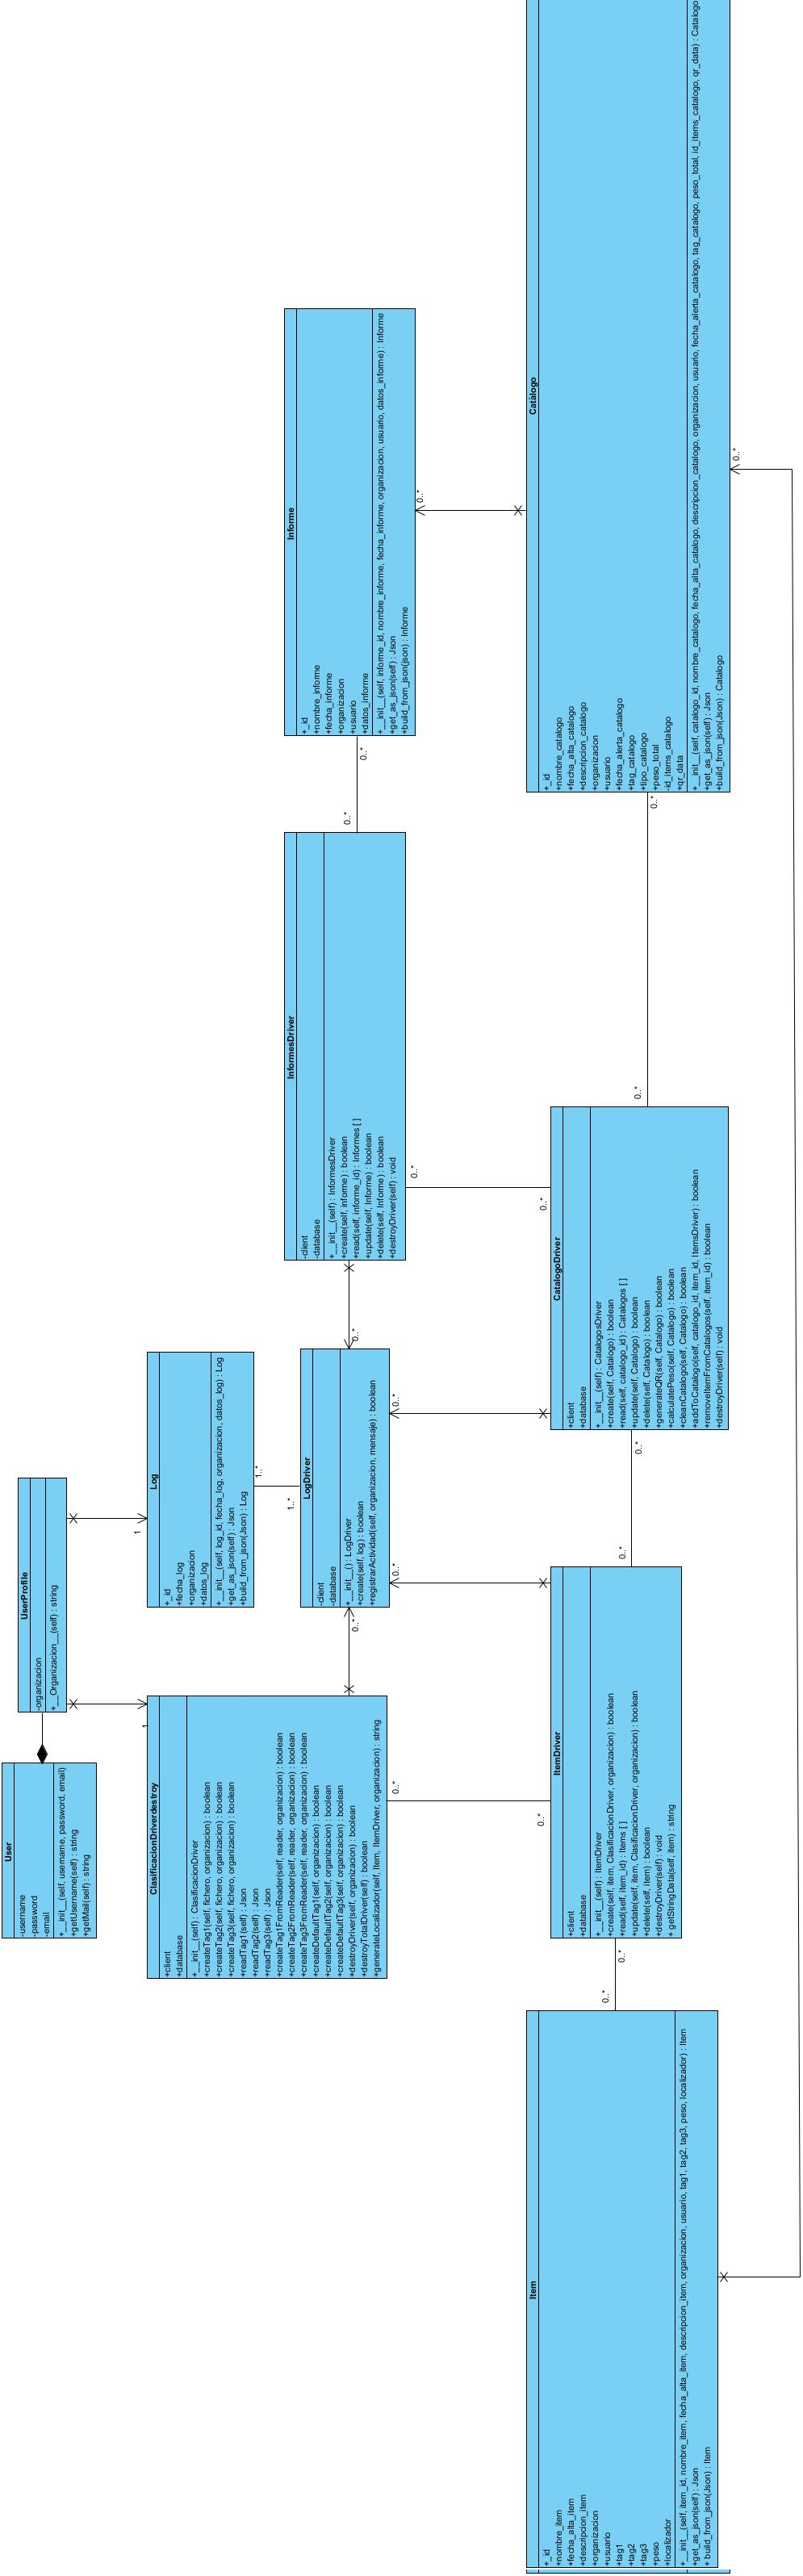
\includegraphics[scale=0.20]{imagenes/clases/NoInventory_clases_web.jpg}
\caption{ Diagrama de Clases - Plataforma Web\cite{propio}  }  
\end{figure}


\section{Analisis Aplicación Android}

\subsection{Requisitos Funcionales Aplicación Android}
Los requisitos funcionales de la aplicación Android establecen los comportamientos o funcionalidades de la aplicación.\\

\textbf{RF-1. Administración de items:} La aplicación deberá administrar los items que formen parte del almacén.   

RF-1.1. La aplicación permitirá detectar items mediante texto o localizador
	
RF-1.2. La aplicación permitirá detectar items mediante código QR
	
RF-1.3. La aplicación permitirá detectar items mediante código de barras
	
RF-1.4. La aplicación permitirá detectar items mediante etiquetas NFC
	
RF-1.5. La aplicación permitirá escribir el localizador de un item en una etiqueta NFC
	
RF-1.6. La aplicación permitirá consultar items
	
RF-1.7. La aplicación permitirá añadir un item detectado a un catálogo determinado
	
RF-1.8. La aplicación permitirá crear items

RF-1.9. La aplicación permitirá eliminar items\\


\textbf{RF-2. Administración de Catálogos:} La aplicación deberá administrar los catálogos que se utilicen para clasificar los items del almacén.\\   

 
	RF-2.1. La aplicación permitirá consultar catálogos.
	
	RF-2.2. La aplicación permitirá añadir items  al catálogo mediante código QR.
	
	RF-2.3. La aplicación permitirá añadir items al catálogo mediante código de barras.

	RF-2.4. La aplicación permitirá añadir items al catálogo mediante etiquetas NFC.
	
	RF-2.5. La aplicación permitirá eliminar items de un catálogo.
	
	RF-2.6. La aplicación permitirá eliminar todos los items de un catálogo
	
	RF-2.7. La aplicación permitirá crear catálogos\\
	
	
\textbf{RF-3. Sesión de Usuario:} La aplicación deberá identificar a cada usuario de manera única para certificar las tareas de administración que se lleven acabo desde la aplicación.\\ 


	RF-3.1. La aplicación permitirá al usuario iniciar sesión.
	
	RF-3.2. La aplicación permitirá al usuario cerrar sesión.
	
	RF-3.3. La aplicación permitirá registrarse al usuario.\\



\subsection{Casos de Uso}
Como ya se comentó anteriormente, los diagramas de casos de uso, determinan el contexto del uso de la aplicación, mostrando el punto de vista de los usuarios  y sus interacciones con el sistema.

\begin{figure}[H]  
\centering 
\includegraphics[scale=0.50]{imagenes/casosUso/gestion_Items_Android.jpg}
\caption{ Casos de uso - Gestión Items Android\cite{diagrama} }  
\end{figure}

\begin{figure}[H]  
\centering 
\includegraphics[scale=0.50]{imagenes/casosUso/gestion_catalogos_android.jpg}
\caption{ Casos de uso - Gestión Catálogos Android\cite{diagrama}  }  
\end{figure}

\begin{figure}[H]  
\centering 
\includegraphics[scale=0.7]{imagenes/casosUso/gestion_usuarios_android.jpg}
\caption{ Casos de uso - Gestión Usuarios Android\cite{diagrama}  }  
\end{figure}


\subsection{Diagramas de Secuencia}
El siguiente punto, recoge los diagramas de secuencia de la aplicación Android,  mostrando las interacciones de la aplicación a través del tiempo. Debido a que la aplicación es una extensión de la plataforma web, se ha optado por obviar algunos diagramas de secuencia, ya que las interacciones entre usuario y sistema tienen el mismo flujo temporal que en la plataforma web. Se considera interesante en lo relativo a la gestión de items, especificar los procesos de detectar o buscar items utilizando el lector de códigos de barras o códigos QR y el lector de etiquetas NFC y también el proceso de escritura del identificador de un item en una etiqueta NFC. 

\begin{figure}[H] 
\centering 
\includegraphics[scale=0.50]{imagenes/secuencia/android/detectar_item_qr_barras.jpg}
\caption{ Diagramas de Secuencia - Detectar Item Lector de Códigos\cite{diagrama}  }  
\end{figure}

\begin{figure}[H] 
\centering 
\includegraphics[scale=0.50]{imagenes/secuencia/android/detectar_item_nfc.jpg}
\caption{ Diagramas de Secuencia - Detectar Item Lector NFC\cite{diagrama}  }  
\end{figure}

\begin{figure}[H] 
\centering 
\includegraphics[scale=0.50]{imagenes/secuencia/android/escribir_nfc.jpg}
\caption{ Diagramas de Secuencia - Escribir Item Etiqueta NFC\cite{diagrama}  }  
\end{figure}

Como parte de los diagramas de secuencia, es interesante especificar en lo relativo a la gestión de catálogos, los procesos de añadir items a un catálogo específico utilizando el lector de códigos de barras o QR o el lector de etiquetas NFC.

\begin{figure}[H] 
\centering 
\includegraphics[scale=0.50]{imagenes/secuencia/android/add_item_barras.jpg}
\caption{ Diagramas de Secuencia - Añadir Item a Catálogo - Lector de Códigos\cite{diagrama}  }  
\end{figure}

\begin{figure}[H] 
\centering 
\includegraphics[scale=0.50]{imagenes/secuencia/android/add_item_nfc.jpg}
\caption{ Diagramas de Secuencia - Añadir Item a Catálogo - Lector NFC\cite{diagrama}  }  
\end{figure}



\subsection{Diagrama de Clases}
Para alcanzar un mayor grado de comprensión de la aplicación Android, se presenta también el siguiente diagrama de clases. 
\begin{figure}[H] 
\centering 
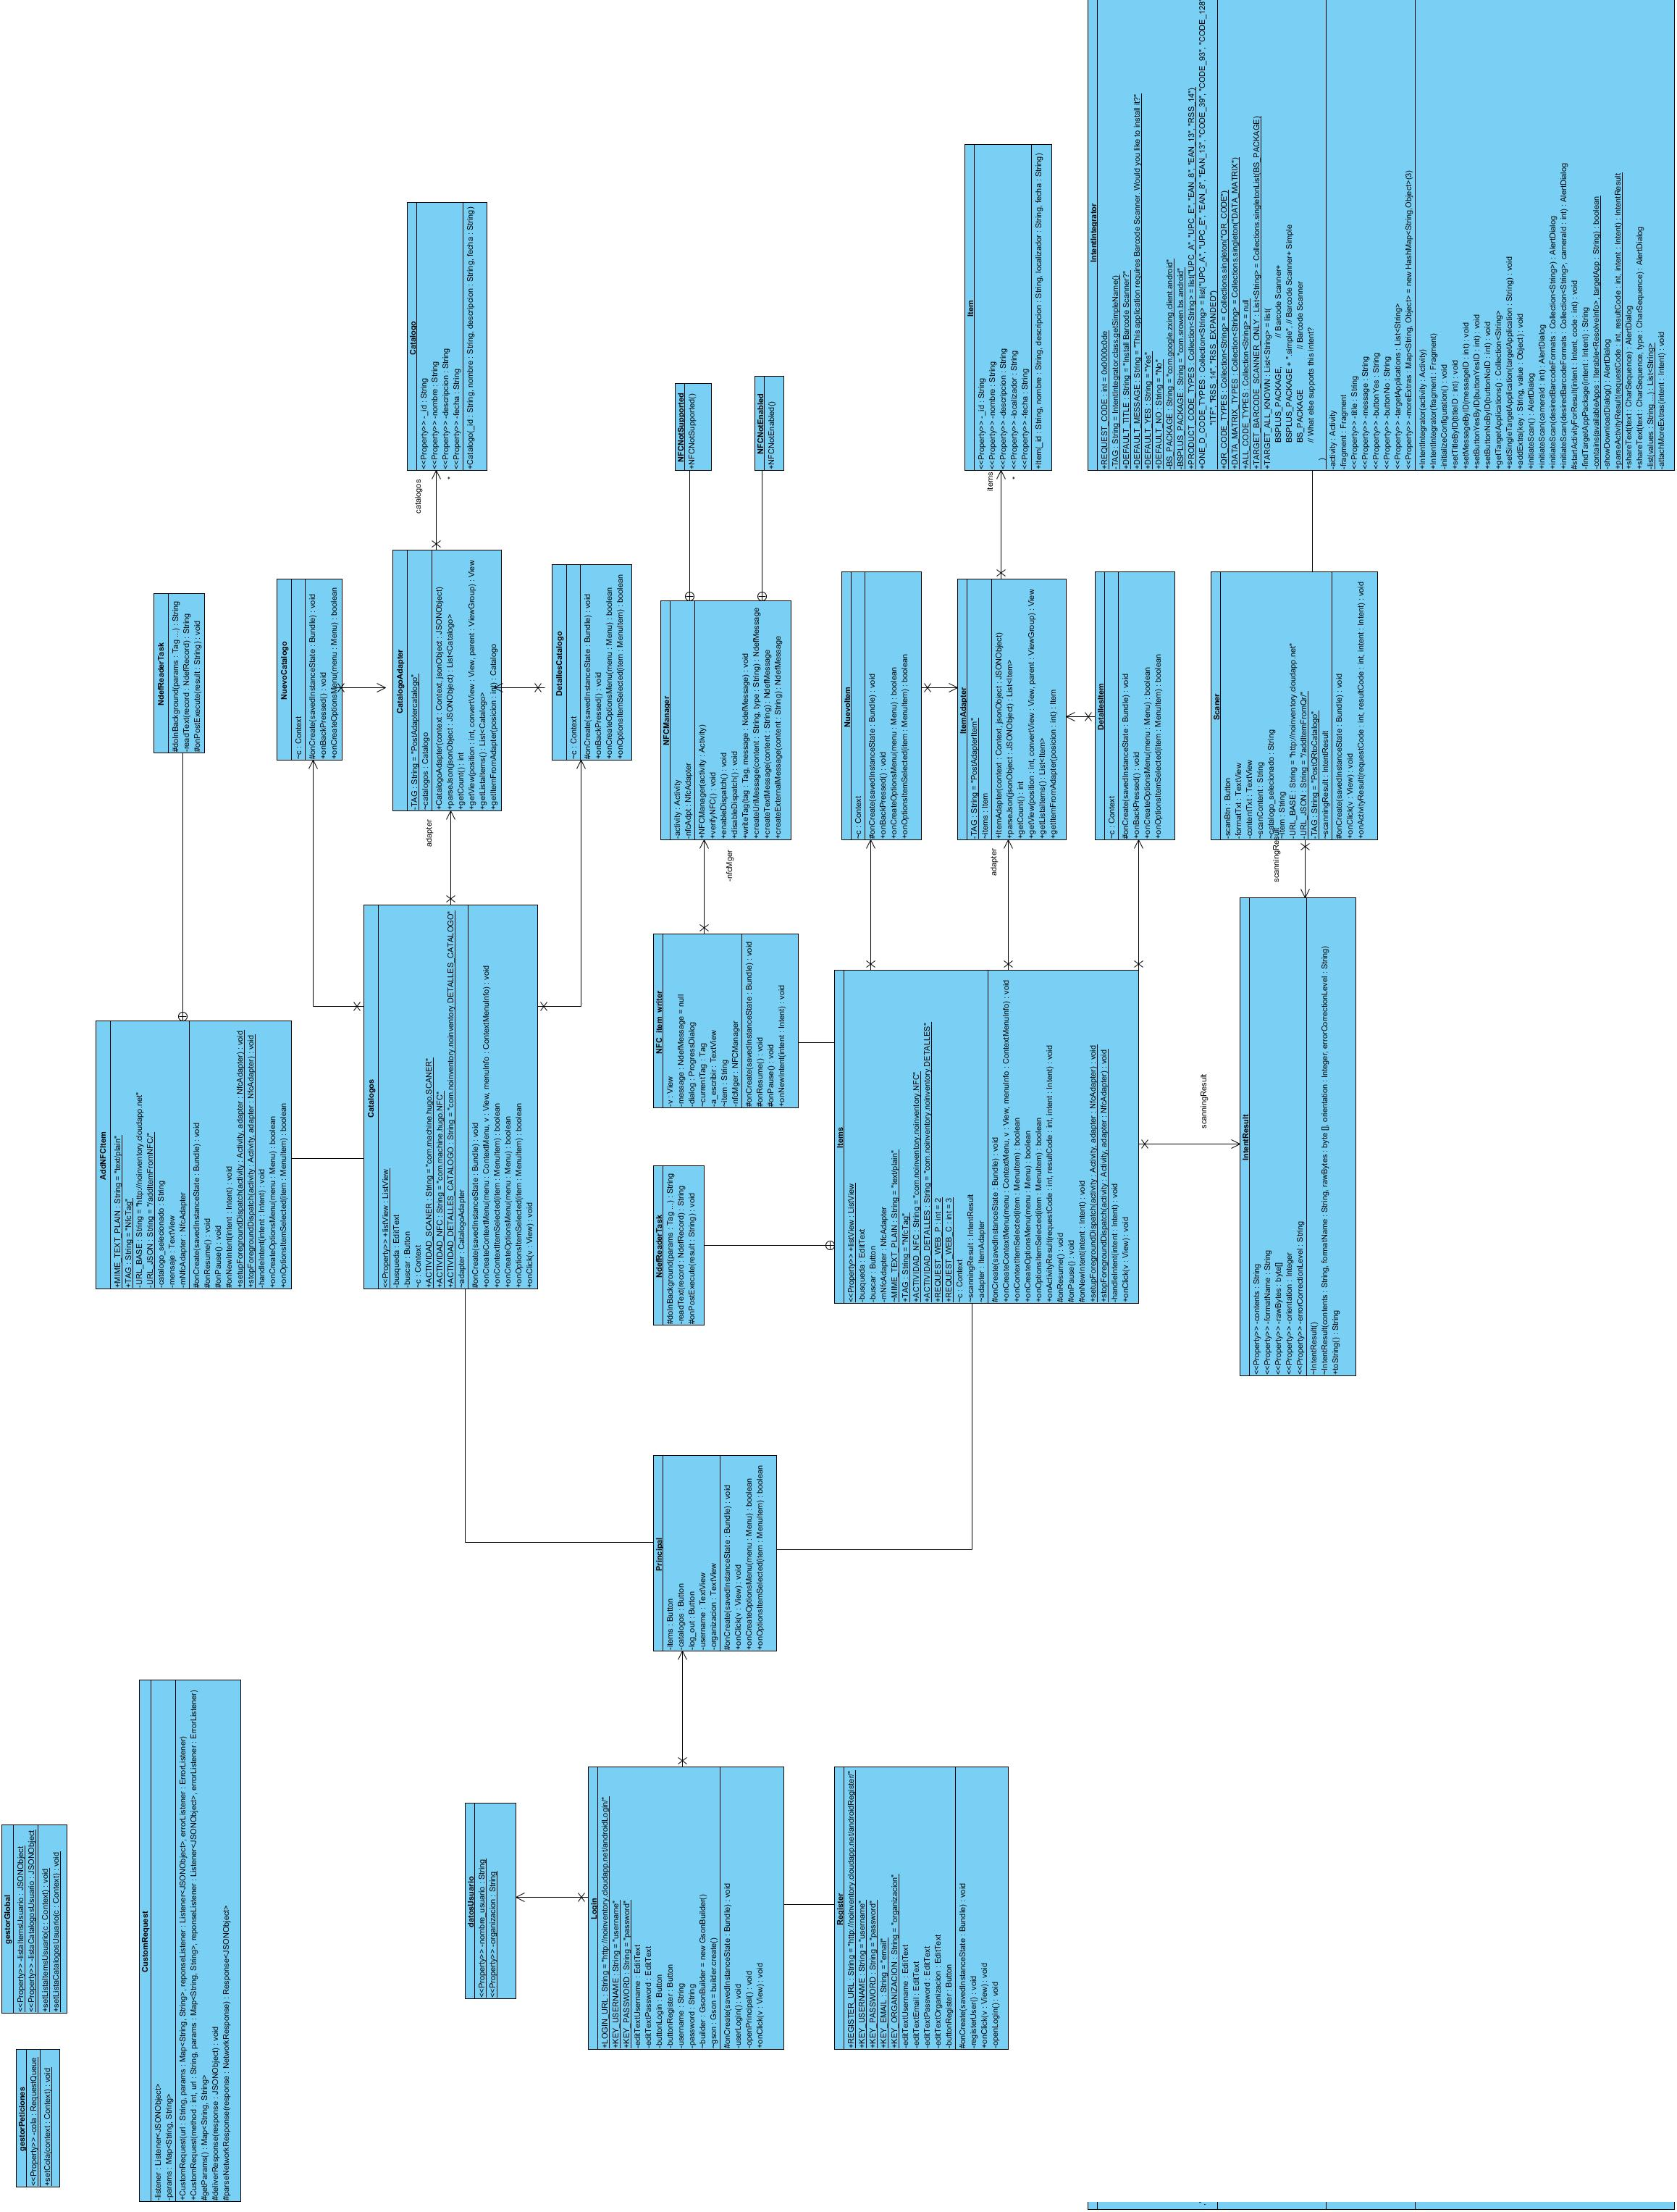
\includegraphics[scale=0.20]{imagenes/clases/clasesAndroid.jpg}
\caption{ Diagrama de Clases - Android\cite{propio}  }  
\end{figure}




\chapter{Desarrollo del Sistema}
En esta parte se abordarán los aspectos más importantes en el desarrollo del sistema. ¿Qué tecnologías has sido utilizadas?, ¿como han sido utilizadas? y ¿por qué han sido utilizadas?
para alcanzar un mayor grado de comprensión, se ha desglosado el proceso de desarrollo en 3 bloques principales: Desarrollo Web, Infraestructura y Desarrollo Android. 


\section{Desarrollo Web}

En el proceso de desarrollo web, se ha seguido el patrón de arquitectura software modelo-vista-controlador (MVC)\cite{mvc} cuya finalidad es separar los datos y la lógica de una aplicación de la interfaz de usuario. Este patrón de arquitectura se basa en la reutilización de código y separación de conceptos con el objetivo de facilitar el desarrollo y mantenimiento de aplicaciones que al utilizar esta metodología son fácilmente escalables. 

\begin{figure}[H] 
\centering 
\includegraphics[scale=0.25]{imagenes/desarrollo_herramienta/mvc.png}
\caption{ Modelo-Vista-Controlador\cite{mvc2}  }  
\end{figure} 

Los componentes\cite{mvc3}\cite{mvc4} del Modelo-Vista-Controlador se pueden definir en:

\begin{enumerate}
\item \textbf{Modelo:} Representa la información , gestiona los accesos a ella, la base de datos seria un componente del modelo. 

\item \textbf{Vista:} Representa el modelo en un formato adecuado para interactuar con él mediante la interfaz de usuario.  

\item \textbf{Controlador:} Responde a eventos invocando peticiones al modelo cuando se hace alguna solicitud de la información (por ejemplo, editar un documento o un registro en una base de datos). El controlador interactúa con su vista asociada para realizar cambios en la forma de representar el modelo. 
\end{enumerate}


Como parte del desarrollo web también se ha utilizado la metodología de ingeniería del software conocida como desarrollo basado en test o TDD. Dicha metodología consiste en escribir los test necesarios para cubrir las funcionalidades de la plataforma web y a partir de ellos, escribir el código necesario para que dichas pruebas sean superadas, cumpliendo así la funcionalidad que se esta poniendo a prueba.  Se profundizará mas en esta metodología en el capítulo 4: Implementación y Pruebas que contiene una sección dedicada al TDD\ref{sec:TDD}

Este proyecto se ha desarrollado en python, utilizando el framework Django. Como sistema de bases de datos, se ha utilizado mongoDB por su capacidad de manejar grandes cantidades de datos y su eficiencia a la hora de realizar consultas, algo imprescindible para el correcto funcionamiento tanto de la web como de la aplicación Android. Para la interacción con este motor de bases de datos se ha utilizado el cliente Pymongo. Para mejorar la experiencia de usuario, se ha utilizado técnicas de programación en el cliente basadas en Ajax, Jquery y Javascript. Para la apariencia de la web, se ha utilizado el framework CSS Bootstrap.La plataforma web también cuenta con diversos servicios externos como son la generación de códigos identificativos y un servicio de correo electrónico. A continuación se profundizará en las herramientas utilizadas en cada una de las partes de la plataforma web.

 



\subsection{Back-End}

El Back-End o lado del servidor es la capa encargada del acceso a los datos. En este proyecto se ha decidido utilizar Django\cite{dj} como framework de alto nivel para trabajar con python en el servidor. Este framework reúne diversas herramientas y aplicaciones, como por ejemplo el servidor de aplicación para desarrollo que facilita el trabajo para desarrollar de manera ágil, el modulo de autenticación de usuarios, el modulo para desarrollo basado en test o la integración de servicios externos como el cliente de mensajería interna. Al principio se planteó realizar la plataforma web en PHP utilizando el framework Symfony pero al ser un sistema bastante grande, se decidió optar por Django ya que facilitaba el proceso de desarrollo. También se pensó en el micro-framework python Flask\cite{fl} pero después del proceso de análisis, se llegó a la conclusión de que con Flask se repetiría mucho más código y con Django el diseño sería más escalable.

\begin{figure}[H] 
\centering 
\includegraphics[scale=0.55]{imagenes/desarrollo_herramienta/django.png}
\caption{ Arquitectura Django\cite{djA}  }  
\end{figure} 

Django sigue la metodología de diseño “ Modelo - Vista - Controlador ” (MVC) lo que permite crear aplicaciones web extensibles, escalables y sostenibles. Django es de código abierto y cuenta con diversos módulos para asegurar la seguridad e integridad de las aplicaciones web desarrolladas en él. 
Django posee un sistema jerárquico de plantillas que facilita la reutilización de código y extensibilidad de aplicaciones. Además cuenta con soporte para internacionalización.
\subsubsection{Sistema Gestor de Bases de Datos}
La parte imprescindible para la capa de acceso a datos es el sistema gestor de bases de datos, encargado de almacenar los modelos del sistema. Como propuesta inicial para el desarrollo del sistema, se pensó en utilizar un esquema relacional utilizando sistemas gestores de bases de datos relacionales como MySQL o PostgreSQL por la manera de realizar las consultas y por la facilidad de diseño entidad-relación pero tras el proceso de análisis, se llego a la conclusión de que utilizando un esquema relacional, no se podría dotar al sistema de la flexibilidad necesaria para satisfacer las necesidades de cada entidad o almacén, ya que este esquema tradicional obliga a que todas las filas de una tabla representativa de un modelo tengan los mismos campos para mantener la entidad referencial del sistema. En vista de este problema, se pensó también utilizar Elasticsearch, herramienta con la que se podría alcanzar el grado de flexibilidad necesaria para los modelos, pero debido a su compleja integración con Django, finalmente se descartó la opción de utilizarla. Debido a esto, se ha decido utilizar MongoDB\cite{mg} como sistema gestor de bases de datos no-relaciones también denominadas bases de datos documentales, con el objetivo de conseguir un esquema interno flexible y eficiente. 

MongoDB es un sistema de base de datos NoSQL orientado a grandes cantidades de datos, guarda estructuras de datos en documentos similares a JSON haciendo que la integración de los datos en ciertas aplicaciones sea más fácil y rápida.
Se trata de una base de datos ágil que permite cambiar los esquemas de una aplicación cuando esta evoluciona. Los principales objetivos de estas bases de datos son la escalabilidad, rendimiento y gran disponibilidad.
En MongoDB los documentos se agrupan en colecciones. Las colecciones  no imponen una estructura fija a los documentos que contienen, ni siquiera al tipo de datos de cada campo. Esto es una ventaja cuando estamos desarrollado un sistema en el que las entradas de la base de datos dependen de las preferencias del usuario.

\begin{figure}[H] 
\centering 
\includegraphics[scale=0.55]{imagenes/desarrollo_herramienta/mongo.jpg}
\caption{ Arquitectura MongoDB\cite{mongoA}  }  
\end{figure} 

Las principales características de las bases de datos no-relacionales como MongoDB son la velocidad y la flexibilidad. La eficiencia en las consultas sobre bases de datos no-relacionales, y mas aun, cuando estas consultas marcan la calidad de experiencia que percibe el usuario, ya sea en el portal web o en la aplicación Android.  Las tareas de consulta, inserción, modificación o borrado presentan una gran eficiencia ya que pueden ser realizadas mediante funciones JavaScript en el cliente, conectando directamente con la base de datos.
En cuanto a la flexibilidad, la principal ventaja es la escalabilidad, por ejemplo, en el momento en que un usuario necesite mas atributos para clasificar sus objetos, lo que en el mundo de las bases de datos relacionales se traduciría en agregar mas columnas a las tablas que representan todos los objetos, cuando se trabaja con bases de datos no relacionales esto no es un impedimento, ya que en la misma colección pueden convivir documentos u objetos con distintos campos o valores. Esto es perfecto para darle al usuario la libertad de personalizar los atributos con los que quiere identificar sus objetos. 
Las consultas sobre MongoDB son consultas Ad Hoc, las cuales soportan búsqueda por campos, consultas por rangos y expresiones regulares. También pueden ser funciones JavasScript definidas por el desarrollador. 
Cualquier documento de MongoDB puede ser indexado. Los índices funcionan de manera similar a los de las bases de datos relacionales. 
En cuanto a la replicación y Balanceo de carga, MongoDb soporta el paradigma maestro-esclavo. Es capaz de escalar horizontalmente y tiene la capacidad de ejecutarse en múltiples servidores, balanceando la carga y duplicando de datos para garantizar el funcionamiento del sistema en caso de fallo. 
En MongoDB, los documentos los guarda en BSON, que es una forma de representar de forma binaria objetos JSON. Un ejemplo de documento almacenado en MongoDB que representa a un item del almacén, es el siguiente:
\begin{lstlisting}
{u'nombre_item': u'nombre del objeto', 
 u'descripcion_item': u'Detalles del objeto', 
 u'tag1': u'Facultad de Filosof\xeda y Letras',
 u'tag2': u'SWITCH',
 u'tag3': u'NO FUNCIONAL',
 u'usuario': u'user',
 u'peso': u'0.0',
 u'organizacion': u'osl',
 u'fecha_alta_item': u'2016-06-02 07:50:41',
 u'localizador': u'010B05140000001',
 u'_id': ObjectId('574fe5511a4d6d0e054d8519')}
\end{lstlisting}
Este documento es básico. Los documentos pueden anidarse, dando lugar a documentos mas complejos con muchas mas información. Pueden contener también listas de otros elementos o valores. 
\subsubsection{Pymongo} 
Para interactuar con MongoDB, se utiliza Pymongo\cite{pymongo}, un paquete python que facilita un cliente o driver intermediario para controlar la iteración del sistema con la base de datos MongoDB. Algunas de las características que Pymongo ofrece son:
\begin{enumerate}
\item Conexión con la Base de Datos
\item Visualización de las Bases de Datos creadas.
\item Creación de nuevas Bases de Datos
\item Visualización de las colecciones creadas
\item Creación de nuevas colecciones
\item Inserción de nuevos documentos
\item Actualización de documentos
\item Búsqueda de documentos
\item Eliminación de documentos
\end{enumerate}
Pymongo es el controlador que permite a nuestro modelos interaccionar con la base de datos, de esta manera se consigue utilizar Django, que esta pensado para bases de datos relacionales, con MongoDB que es una base de datos no relacional ya que funciona como intermediario entre los modelos de objetos creados de manera externa al framework y la base de datos.


 
\subsection{Front-End}

El Front-End, capa de presentación o capa de cliente es la encargada de maquetar la estructura semántica del contenido, codificar el diseño en hojas de estilo y controlar la interacción con el usuario. En este proyecto la programación en el lado cliente juega un papel importante a la hora de mejorar la experiencia del usuario en la plataforma, manteniendo los datos actualizados en función de las actualizaciones de los distintos usuarios que trabajan en un mismo entorno colaborativo. La forma de trabajar en el cliente es mediante llamadas asíncronas al servidor, utilizando JQuery y Ajax para realizar llamadas asíncronas al servidor.  

\subsubsection{JQuery y Ajax}

JQuery\cite{jq} es una librería de JavaScript, que permite interactuar con los documentos HTML, manipular el árbol DOM, manejar eventos, desarrollar animaciones y agregar interacción con el servidor mediante llamadas asíncronas realizadas con Ajax. Su objetivo principal es dar un comportamiento dinámico a las paginas web. Jquery funciona en múltiples navegadores, ya que es compatible con CSS3.  

Ajax\cite{aj}, abreviatura de JavaScript Asíncrono y XML es un conjunto de técnicas de desarrollo web en el cliente para crear aplicaciones asíncronas y dinámicas. Con Ajax, las aplicaciones web pueden enviar y recibir datos desde el servidor en segundo plano sin que interfiera en la visualización o el comportamiento de la aplicación. Utilizar Ajax supone crear aplicaciones web en las que la capa de intercambio de datos ha sido separada de la capa de presentación, lo que permite un comportamiento dinámico sin la necesidad de recargar el navegador. 

\begin{figure}[H] 
\centering 
\includegraphics[scale=0.35]{imagenes/desarrollo_herramienta/ajax.png}
\caption{ Modelo Ajax\cite{aj2}  }  
\end{figure}   

En este proyecto, el principal uso de Jquery se realiza junto con Ajax para recargar la información de la web de manera dinámica mediante llamadas asíncronas. El uso de estas tecnologías mejora la experiencia del usuario cuando interactúa con el sistema mediante la plataforma web y la aplicación Android.


\subsubsection{Bootstrap}
Bootstrap\cite{boo} es un framework CSS para dar forma a sitios web mediante librerías CSS. Bootstrap  permite crear interfaces de usuario limpias y totalmente adaptables a todo tipo de dispositivos y pantallas ya que esta caracterizado por ser responsive. Es compatible con los siguientes navegadores: 

\begin{enumerate}
\item Google Chrome
\item Safari
\item Mozilla Firefox 
\item Internet Explorer 
\item Opera  
\end{enumerate}
  
\subsection{Herramientas y Servicios}
Para dotar a la plataforma de diversas funcionalidades, se han incluido ciertos servicios externos. 

\subsubsection{SendGrid}
SendGrid\cite{sg} es un servicio cloud de correo electrónico. Proporciona un sistema de entrega de correos electrónicos transaccional. SendGrid cuenta con una API flexible que facilita la integración personalizada del servicio. 
 

En este proyecto, se ha utilizado SendGrid para implantar un buzón de incidencias en la página principal. Dicho buzón, permite a los usuarios interesados, contactar con el administrador del sistema en caso de incidencia o en caso de necesitar información. Dicho buzón también permite contactar con los usuarios registrados que pertenecen a alguna organización o almacén en concreto. Al utilizar Django como marco de trabajo la integración de  SendGrid  es muy sencilla. Es necesario disponer de una cuenta en el servicio y añadir las siguientes lineas al archivo de configuración settings.py de Django:
\begin{lstlisting}
EMAIL_HOST = 'smtp.sendgrid.net'
EMAIL_HOST_USER = os.environ.get('MAIL_USER')
EMAIL_HOST_PASSWORD = os.environ.get('MAIL_PASS')
EMAIL_PORT = 587
EMAIL_USE_TLS = True
\end{lstlisting}
El nombre de usuario y la contraseña son establecidas mediante variables de entorno para garantizar la seguridad del servicio. SendGrid facilita de manera gratuita, cuentas con 25.000 correos electrónicos gratuitos cada mes.

\subsubsection{Generación de Identificadores }

Para la generación de códigos QR, se ha decidido utilizar la API  Google Charts\cite{googleqr} creando con ella un template tag de Django. Este template recibe como argumento dos cadenas de texto, una el identificador de objeto y otra la alternativa a mostrar en caso de que no sea posible generar la imagen con el código QR. 

\begin{lstlisting}
@register.filter
@stringfilter
def qrcode(value, alt=None):
    """
    Generate QR Code image from a string with the Google charts API
    Ejemplo de Uso -->  {{ my_string|qrcode:"my alt" }}
    <img src="http://chart.apis.google.com/chart?chs=150x150&amp;cht=qr&amp;chl=my_string&amp;choe=UTF-8" alt="my alt" />
    """
    url = conditional_escape("http://chart.apis.google.com/chart?%s" % \
            urllib.urlencode({'chs':'200x200', 'cht':'qr', 'chl':value, 'choe':'UTF-8'}))
    alt = conditional_escape(alt or value)

    return mark_safe(u"""<img class="qrcode" src="%s" width="200" height="200" alt="%s" />""" % (url, alt))
\end{lstlisting}

Para la generación de códigos de barras se procede de la misma forma, pero utilizando el generador gratuito de códigos de barras MBCEStore\cite{barras} 

\begin{lstlisting}
@register.filter
@stringfilter
def barcode(value, alt=None):
    #{{ my_string|barcode:"my alt" }}#
    url='http://www.mbcestore.com.mx/generador_codigo_de_barras/codigo_de_barras.html?code='+value+'&style=197&type=C128B&width=250&height=50&xres=1&font=4'
    alt = conditional_escape(alt or value)
    return mark_safe(u"""<img class="barcode" style="border-radius: 0px" src="%s"  alt="%s" />""" % (url, alt))
\end{lstlisting}

\subsubsection{Github}
GitHub es una plataforma de desarrollo colaborativo de software para alojar proyectos utilizando el sistema de control de versiones Git. El código es almacenado de forma pública o privada. GitHub aloja tu repositorio de código y te brinda herramientas muy útiles para el trabajo en equipo, dentro de un proyecto. Github ofrece varias herramientas:

\begin{enumerate}
\item Una wiki para el mantenimiento de las distintas versiones de las páginas. 
\item Un sistema de seguimiento de problemas que permiten a los miembros de tu equipo detallar un problema con tu software.
\item Una herramienta de revisión de código, donde se pueden añadir anotaciones en cualquier punto de un fichero y debatir sobre determinados cambios realizados en un commit específico. 
\item Un visor de ramas donde se pueden comparar los progresos realizados en las distintas ramas de un repositorio. 
\end{enumerate}

Como parte del desarrollo de este proyecto, se ha utilizado Github como plataforma para el control de versiones. Github también ha sido utilizado para la automatización de tareas. Como se verá en la siguiente sección, el repositorio del proyecto esta vinculado con algunas herramientas cloud, de manera que al realizar push sobre el proyecto, estas herramientas cloud lanzan disparadores para integración continua, automatizar despliegues en PaaS o generar imágenes Docker. Todo esto se verá en detalle en la siguiente sección, dedicada a la infraestructura del proyecto. Los repositorios en los que están alojados los fuentes del proyecto son los siguientes:   

 
\section{Infraestructura}

En esta sección se detallará la infraestructura virtual subyacente con la que cuenta el proyecto. Para empezar se hablará de las herramientas de integración continua utilizadas y el papel que juegan en el despliegue. Se hablará también de Heroku, la Plataforma como servicio utilizada, de como distribuir la base de datos MongoDB utilizando Mlab. También se hablará de Azure, la infraestructura como servicio utilizada, de las herramientas de despliegue utilizadas para trabajar con Azure y por último como utilizar Docker y las ventajas del aislamiento de recursos para levantar instancias del sistema de manera rápida en el caso de que la cantidad de datos a gestionar por el cliente así lo requiera. 

\subsection{Integración Continua}

Para detallar la infraestructura subyacente con la que cuenta el proyecto, es necesario comenzar hablando de las herramientas de integración continua que se usan en el. La integración continua consiste en realizar compilaciones y ejecución de pruebas o test unitarios de todo el proyecto, cada cierto tiempo con el objetivo de detectar fallos. Debido al desarrollo TDD, el proyecto cuenta con las baterías de test asociadas a los modelos y a sus manejadores.

\subsubsection{Travis-CI}
En este proyecto la primera herramienta de integración continua utilizada es Travis-CI\cite{travis}.Travis es un  sistema distribuido de integración continua utilizado para construir y testear proyectos. Travis utiliza el control de versiones GitHub y un archivo denominado travis.yml\ref{sec:travis} para realizar el proceso de integración. En dicho fichero, se especifica el lenguaje utilizado, la versión, la instalación de dependencias y la ejecución de test unitarios. Dicho fichero también puede utilizarse para realizar despliegue de la aplicación en distintas plataformas aunque en este proyecto no ha sido el caso. Travis es una herramienta de código abierto compatible con multitud de lenguajes. 

\subsubsection{SNAP-CI}
La segunda herramienta de integración continua utilizada ha sido SNAP-CI\cite{snap}. Esta herramienta es perfecta para el proceso de integración continua y la automatización del despliegue de la aplicación. Como podemos observar en la siguiente imagen, Snap-CI nos permite vincular el repositorio de github en el que se encuentra el sistema y desglosar en un pipeline los distintos pasos que de pasar la aplicación para completar la integración y desplegarse.En este proyecto, el pipeline esta desglosado en 3 bloques, los cuales se ejecutarán cada vez que se realice un push al repositorio:

\begin{enumerate}
\item Instalación de dependencias
\item Ejecución de los test unitarios
\item Despliegue en un PaaS (Heroku)  
\end{enumerate}

\begin{figure}[H] 
\centering 
\includegraphics[scale=0.30]{imagenes/desarrollo_herramienta/snp_ci.png}
\caption{ Pipeline Snap-CI\cite{snapP}  }  
\end{figure}  	





\subsection{Plataforma Como Servicio}

Para continuar con el desarrollo de la infraestructura, se va a hablar de la plataforma como servicio. Como se vio en la introducción, la plataforma como servicio es uno de los servicios cloud que hoy en día pueden ofrecerse. Este proyecto se encuentra desplegado en el PaaS Heroku\cite{hero} que al ser de carácter gratuito el objetivo de desplegar el sistema aquí es tener una versión disponible para que el usuario prueba el sistema sin ningún compromiso.
 	
 

Heroku es una plataforma en la nube basado en un sistema de contenedores gestionados, con servicios de datos integrados y un potente ecosistema, para implementar y ejecutar aplicaciones. Heroku presenta una fácil integración con github y con herramientas de integración continua como vimos en la subsección anterior. Heroku se caracteriza por el fichero de configuración denominado Procfile. Dicho fichero, se encarga de arrancar una instancia web y dejar que gunicorn (servidor de aplicación) ejecute el sistema en ella. Heroku también cuenta con una herramienta de linea de comandos que facilita la automatización de tareas y despliegues. 

El principal problema es que Heroku es gratuito hasta cierto punto, por ejemplo el sistema de bases de datos es de pago, por lo que se decidió utilizar Mlab para distribuir la base de datos.

Mlab\cite{mlab} es un servicio de base de datos alojado en la nube completamente gestionado que proporciona servicio de bases de datos MongoDB. MLab se ejecuta en proveedores cloud como Amazon, Google y Microsoft Azure. Mlab facilita la automatización de despliegue, proporciona servicio de Backup, Recovery, monitorización y alertas de consumo desde la interfaz del navegador. Mlab proporciona de manera gratuita hasta 500MB de almacenamiento y el acceso a las bases de datos creadas en la plataforma se realiza mediante url la cual aprovechan los clientes de bases datos como Pymongo para conectar con el servicio, de esta manera se consigue distribuir la base de datos cuando estamos trabajando por ejemplo con Heroku. 

\begin{figure}[H] 
\centering 
\includegraphics[scale=0.95]{imagenes/desarrollo_herramienta/mlab.png}
\caption{ Mlab - Native REST interface\cite{mlabL}  }  
\end{figure} 
  

\subsection{Infraestructura Como Servicio}
Para finalizar con el desarrollo de la infraestructura, se va a hablar de la infraestructura como servicio. Como se vio en la introducción, la infraestructura como servicio es uno de los servicios cloud que proporciona acceso a recursos informáticos situados en un entorno virtualizados. Este proyecto, a nivel de IaaS, se encuentra desplegado en Azure\cite{azure} con el objetivo de  dar la mejor experiencia, calidad de servicio y alta disponibilidad al usuario, ya que al no necesitar distribuir la base de datos, la eficiencia se ve incrementada de manera importante.
Azure proporciona herramientas integradas, plantillas precompiladas e infinidad de servicios administrados para facilitar la compilación y administración de aplicaciones. Azure admite una gran selección de sistemas operativos, lenguajes de programación, frameworks, bases de datos y dispositivos. Proporciona una gran flexibilidad a través de su red de conexiones privadas seguras, y sistemas de almacenamiento híbridos pagando solo por su uso. 

\begin{figure}[H] 
\centering 
\includegraphics[scale=0.50]{imagenes/desarrollo_herramienta/azure.png}
\caption{ Arquitectura Azure\cite{azureA}  }  
\end{figure}

Al trabajar con Azure a nivel de IaaS, disponemos de maquinas virtuales en linea con la capacidad de dar servicio y con la posibilidad de instalar en ellas todo lo que el sistema necesite para funcionar de manera óptima. En las siguientes subsecciones se detallarán las herramientas utilizadas en este proyecto para configurar estas maquinas en función del tipo de servicio que se quiera ofrecer. 

\subsubsection{Vagrant}

La herramienta base es Vagrant\cite{vg}, herramienta open-source para la creación y configuración de entornos de desarrollo virtualizados. Vagrant proporciona entornos de trabajo fáciles de configurar, reproducibles y portátiles. Está desarrollado con Ruby y utiliza el sistema de virtualización Virtualbox de Oracle. Este proyecto tiene asociado un fichero denominado Vagrantfile\ref{sec:vagrantfile} cuya función principal es la de describir el tipo de máquinas necesarias para la aplicación, cómo configurarlas y como aprovisionarlas. Las posibilidades con Vagrant son muy numerosas, en este proyecto se va a utilizar Vagrant para la configuración de maquinas virtuales alojadas en Azure. Dichas maquinas correrán directamente con la aplicación utilizando Ansible y también correrán con la aplicación de manera asilada utilizando contenedores. 

\begin{figure}[H] 
\centering 
\includegraphics[scale=0.95]{imagenes/desarrollo_herramienta/vagrant.jpeg}
\caption{ Funcionamiento Vagrant\cite{vg2}}
\end{figure}


Dependiendo del proveedor de servicio, Vagrant será configurado de una manera u otra. En este proyecto se ha utilizado Azure, por lo que Vagrant necesita el plugin Microsoft Azure provider to Vagrant. Con este plugin detallamos entre otras cosas las credenciales necesarias para autenticación en Azure.

Vagrant cuenta con infinidad de plugins para distintos cloud services y distintos entornos de de desarrollo virtuales. Con Vagrant no solo podemos trabajar individualmente maquina a máquina, podemos utilizar la caracteristica vagrant-multimachine para crear en paralelo N máquinas virtuales y aprovisionarlas cada una como queramos. 


\subsubsection{Ansible}

Ansible\cite{ans} es una herramienta de automatización que permite configurar sistemas, implementar software y orquestar tareas complejas como por ejemplo despliegues continuos. En este proyecto se ha decidido utilizar Ansible como mecanismo de aprovisionamiento de aplicación, debido a su fiabilidad, facilidad de uso y seguridad. Para poder trabajar con Ansible es necesario crear playbooks\ref{sec:playbook} que no son mas que archivos de aprovisionamiento.yml en los que detallar todas las dependencias, servicios y tareas que nuestra aplicación necesita para funcionar. Aunque puede usarse de manera independiente, si la combinamos con herramientas de creación y administración de entornos virtuales como por ejemplo Vagrant, podemos llegar a conseguir grandes resultados.

\begin{figure}[H] 
\centering 
\includegraphics[scale=0.35]{imagenes/desarrollo_herramienta/ansible.jpg}
\caption{ Arquitectura Ansible\cite{ans2}}
\end{figure}



\subsubsection{Docker}

Docker\cite{dk} es una herramienta para automatizar el despliegue de aplicaciones dentro de contenedores, proporcionando una capa de abstracción y automatización de Virtualización a nivel de sistema operativo. Docker utiliza aislamiento de recursos del kernel de Linux, para permitir que contenedores independientes se ejecuten dentro de una sola instancia de Linux, evitando la sobrecarga de iniciar y mantener máquinas virtuales.

\begin{figure}[H] 
\centering 
\includegraphics[scale=0.35]{imagenes/desarrollo_herramienta/docker.png}
\caption{ Virtualización Docker\cite{dkw}}
\end{figure}

La principal diferencia con respecto a maquinas virtuales es el tamaño. Las maquinas virtuales incluyen la aplicación, el codigos, las librerias necesarias y un sistema operativo anfitrion completo mientras que los contenedores contienen los mismo pero comparten el nucleo con otros contenedores corriendo como una proceso asilado en el espacio de usuario del sistema operativo anfitrion. No estan vinculados con ninguna infraestructura especifica 


En este proyecto se ha decidido utilizar Docker con el objetivo de levantar instancias del sistema de manera rápida y asilada. Esto puede ser de gran ayuda a la hora de que el sistema tenga que gestionar un almacén con una cantidad inmensa de elementos. Manejar tal cantidad de datos, podría afectar negativamente no solo al almacén en cuestión, si no a otros usuarios de otros almacenes que obtengan servicio de la misma instancia. Usar Docker puede resultar interesante también cuando los objetos a gestionar sean sensibles y el cliente requiera mayor grado de seguridad para sus datos. Docker también facilita la puesta en producción de la aplicación, ya que en un mismo archivo de configuración denominado Dockerfile\ref{sec:dockerfile}, se pueden automatizar las tareas de puesta en producción, configuración de Nginx\ref{sec:nginx} como servidor de contenido estático, configuración de gunicorn como servidor de aplicación y monitorización del sistema utilizando supervisor\ref{sec:supervisor}. 

Otra ventaja de utilizar Docker es el uso de Docker Hub\cite{dkh}, servicio cloud para la construcción y envío de aplicaciones o servicios utilizando contenedores. Proporciona recursos centralizados para la creación, distribución y gestión de imágenes de contenedores. Permite al usuario la automatización del flujo de trabajo a lo largo de la línea de desarrollo.

Con Docker Hub se vincula el repositorio del proyecto alojado en el control de versiones Github, de manera que cuando se realice un push al repositorio, el servicio detectará el Dockerfile principal, lo ejecutará y generará una imagen preconstruida de la aplicación, con esta imagen se pueden levantar nuevas instancias de la aplicación en cuestión de minutos. 


\begin{figure}[H] 
\centering 
\includegraphics[scale=0.35]{imagenes/desarrollo_herramienta/dockerhub.png}
\caption{ Generación Imagen Docker Hub\cite{dkh2}}
\end{figure}


\section{Desarrollo Android}

Android es un sistema operativo basado en el núcleo Linux diseñado inicialmente para teléfonos móviles, al igual que iOS, Symbian y Blackberry OS. El sistema permite programar aplicaciones en una variación de Java llamada Dalvik. El sistema operativo proporciona todas las interfaces necesarias para desarrollar aplicaciones que accedan a las funciones del teléfono. 

\begin{figure}[H] 
\centering 
\includegraphics[scale=0.5]{imagenes/desarrollo_herramienta/android.png}
\caption{ Arquitectura Android\cite{arqAndroid}}
\end{figure}

Como parte del desarrollo Android, se ha utilizado el paradigma de programación orientada a objetos (POO)\cite{ood}. La característica principal de este paradigma es la unión de datos de entrada y procesamiento en entidades denominadas objetos,  relacionadas a su vez con otras entidades objetos para producir salidas. En función del lenguaje de programación utilizado, existen conjuntos de objetos pre-diseñados que cumplen funcionalidades especificas y que están agrupados en librerías con el objetivo de ahorrar trabajo a los programadores.


\begin{figure}[H] 
\centering 
\includegraphics[scale=0.35]{imagenes/desarrollo_herramienta/pdo.jpg}
\caption{ Diagrama POO\cite{poo}}
\end{figure}


Las principales técnicas de la POO se pueden clasificar en:


\begin{enumerate}
\item \textbf{Herencia:} Permite a los desarrolladores crear nuevos objetos o clases partiendo de una clase o jerarquía de clases ya existente con el objetivo de reutilizar código y extenderlo. 
\item \textbf{Cohesión:} Establece el grado con el que los elementos de un modulo software están relacionados entre si. El objetivo de la cohesión es generar aplicaciones robustas, fiables, reutilizables y facilitar la comprensión de las mimas.
\item \textbf{Abstracción:} Consiste en aislar un elemento de su contexto. Expresa las características esenciales de un objeto, las cuales distinguen al objeto de los demás estableciendo limites conceptuales.
\item \textbf{Polimorfismo:} Propiedad por la que es posible enviar mensajes sintácticamente iguales a objetos de tipos distintos. La única restricción es que los objetos han de ser capaces de contestar al mensaje. 
\item \textbf{Acoplamiento:} es la forma o nivel de interdependencia entre módulos de software. 
 Encapsulamiento: Es el ocultamiento del estado, es decir, de los datos que representan un objeto de manera que sólo se pueda modificar mediante las operaciones propias del objeto.
\end{enumerate}


Resulta interesante conocer el ciclo de vida\cite{col} de las actividades dentro de la aplicación. Una aplicación en Android está formada por un conjunto de elementos básicos de interacción con el usuario, conocidos como actividades y un conjunto de servicios. Una aplicación Android se ejecuta dentro de su propio proceso Linux. Este proceso se crea con la aplicación y continuará vivo hasta que ya no sea necesario y el sistema reclame su memoria para asignársela a otra aplicación. El ciclo de vida de una actividad Android representa las transiciones por las que puede pasar dicha actividad. Las actividades se gestionan como una pila, es decir, desde una actividad se puede llamar a otra, y cuando esta finaliza se vuelve a la actividad invocadora. Las actividades Android pueden pasar por los siguientes estados:

\begin{enumerate}
\item \textbf{Running o Activa:} La actividad está encima de la pila, lo que quiere decir que es visible y tiene el foco.
\item \textbf{Paused o Visible:} La actividad es visible pero no tiene el foco. 
\item \textbf{Stopped o Parada:} Cuando la actividad no es visible. 
\item \textbf{Destroyed o Destruida:} Cuando la actividad termina al invocar el método finish(), o es finalizada por el sistema. 
\end{enumerate}

\begin{figure}[H] 
\centering 
\includegraphics[scale=0.6]{imagenes/desarrollo_herramienta/ciclo_android.png}
\caption{ Ciclo de Vida Actividades Android\cite{colD}}
\end{figure}

Cada vez que una actividad cambia de estado se generan eventos que pueden ser capturados por métodos de la actividad con el objetivo de modelar el comportamiento de la aplicación. Dichos métodos pueden ser: 
\begin{enumerate}
\item \textbf{onCreate():} Se llama en la creación de la actividad. Se utiliza para realizar todo tipo de inicializaciones, como la creación de la interfaz de usuario o la inicialización de estructuras de datos. 
\item \textbf{onStart():} Nos indica que la actividad está a punto de ser mostrada al usuario.
\item \textbf{onResume():} La actividad va a comenzar a interactuar con el usuario. 
\item \textbf{onPause():} La actividad va a ser lanzada a segundo plano, normalmente porque otra actividad es lanzada. 
\item \textbf{onStop():} La actividad ya no va a ser visible para el usuario. En caso de que sean necesarios los recursos del sistema, es posible que la actividad se destruya sin llamar a este método.
\item \textbf{onRestart():} Indica que la actividad va a volver a ser representada después de haber pasado por onStop().
\item \textbf{onDestroy():} Se llama antes de que la actividad sea totalmente destruida. Por ejemplo, cuando el usuario pulsa el botón de volver o cuando se llama al método finish(). Ocurre igual que en el método onStop() y en el caso de que el sistema necesite mas recursos, la actividad puede ser destruida sin llamar a este método. 
\end{enumerate}

Por último, señalar que el desarrollo Android también se basa en el patrón de arquitectura software modelo-vista-controlador (MVC). En dicho patrón, el modelo esta representado por los modelos creados en el Back-End, la vista hace referencia a la interfaz de usuario representada por los ficheros XML y el controlador o lógica de la aplicación por las clases Java. 


En este proyecto, se ha utilizado Android-Studio como entorno de desarrollo para la aplicación. La aplicación se encarga de autenticar a los usuarios y llevar a cabo las tareas de gestión, con el objetivo de poder realizarlas desde el propio almacén. La aplicación consiste en listas de  objetos (items y catálogos), actualizadas periódicamente mediante peticiones HTTP al servidor, para mantener el estado actual del inventario de la organización para la que trabaja el cliente. La aplicación funciona como lector/escritor de etiquetas NFC o como lector de códigos de barras o códigos QR, es decir, realiza las funciones de clasificación a modo de escanear, en función del método de identificación elegido. Ambos métodos (NFC o códigos) son compatibles dentro de una misma organización o almacén, facilitando el trabajo y ahorrando tiempo en las tareas de gestión e identificación. En las siguientes sub-secciones de detallará en profundidad el entorno de desarrollo además de las tecnologías utilizadas como método de identificación. 
 
  

\subsection{Android-Studio}

Para trabajar con Android hay diversos entornos de desarrollo como por ejemplo Eclipse, pero el mas recomendado y el utilizado en este proyecto es Android Studio\cite{as}. Android Studio es un entorno de desarrollo integrado (IDE), basado en IntelliJ IDEA de la compañía JetBrains,  que proporciona varias mejoras con respecto al plugin ADT (Android Developer Tools) para Eclipse. Android Studio utiliza una licencia de software libre Apache 2.0




Algunas características\cite{as2} de este entorno de programación son:

\begin{enumerate}
\item Soporte para programar aplicaciones para Android Wear.
\item Herramientas Lint para detectar problemas de rendimiento, usabilidad y compatibilidad de versiones.
\item Utiliza ProGuard para optimizar y reducir el código del proyecto al exportar a APK.\item Integración de la herramienta Gradle encargada de gestionar y automatizar la construcción de proyectos.
\item Nuevo diseño del editor con soporte para la edición de temas. 
\item Nueva interfaz específica para el desarrollo en Android.
\item control de versiones accediendo a un repositorio desde el que poder descargar Mercurial, Git, Github o Subversion. 
\end{enumerate}

\subsection{Librería Volley}
La aplicación No-inventory-Android-App, sirve como extensión de la plataforma web. Esta aplicación esta sincronizada en tiempo real con el servidor de manera que la experiencia de usuario entre la web y la aplicación es óptima.  Para conseguir esto, se utiliza la librería Volley\cite{volley} desarrollada por Google con el objetivo de optimizar el envío de peticiones Http desde las aplicaciones Android hacia servidores externos. La comunicación Http, hace referencia a las transferencias de hipertexto utilizando el protocolo Hypertext Transfer Protocol o HTTP\cite{http}. Este protocolo de información, permite las trasferencias de información a través de internet. Es un protocolo orientado a transacciones que sigue un esquema petición-respuesta entre un cliente y un servidor. 

\begin{figure}[H] 
\centering 
\includegraphics[scale=0.75]{imagenes/desarrollo_herramienta/HTTP.png}
\caption{ HTTP Esquema\cite{httpD}}
\end{figure}

Volley actúa como una interfaz de alto nivel, liberando al programador de la administración de hilos y procesos de parsing. 


\begin{figure}[H] 
\centering 
\includegraphics[scale=0.5]{imagenes/desarrollo_herramienta/volley.png}
\caption{ Arquitectura Volley\cite{volley2}}
\end{figure}

Volley funciona mediante una arquitectura a capas, en la que cada capa está representada por una hebra. Se puede distinguir entre la hebra principal de la aplicación, la hebra de cache y la hebra que se encarga de realizar las peticiones HTTP.  Las peticiones son añadidas a una cola con prioridad y van siendo atendidas en función de los requisitos de la hebra principal. En el caso de que los datos no estén cacheados, la hebra de cache envía la petición a la hebra de transacción y esta realiza la petición. Un problema importante a la hora utilizar Volley en esta aplicación fue la congestión de la red, ya que cada petición Volley creaba una cola de peticiones propia para cada consulta. La solución tomada fue la de implementar esta cola como estática de manera que todas las peticiones que se llevan a cabo en las distintas vistas de la aplicación, comparten la cola de peticiones, mejorando así el rendimiento y evitando problemas de sobre carga de memoria ya que Volley lo cachea todo. 


\subsection{Near field communication (NFC)}
NFC\cite{nfc} o comunicación de campo cercano, es una tecnología inalámbrica derivada de la etiquetas RFID. NFC es una plataforma abierta pensada para teléfonos  y dispositivos móviles. Su tasa de trasferencia ronda entono a los  424 kbit/s por lo que es ideal para la comunicación instanatea aunque como su propio nombre indica, su radio de acción esta entorno a los 10 o 15 cm aunque no necesita emparejamiento previo. 

La tecnología NFC puede funcionar en dos modos:

\begin{enumerate}
\item Activo, en el que ambos equipos con NFC intercambian datos. 
\item Pasivo, en el que solo hay un dispositivo activo y el otro aprovecha el campo magnético generado por este para intercambiar la información.
\end{enumerate}

En este sistema, la aplicación No-inventory-Android-App es capaz de Leer/Escribir etiquetas NFC. Dichas etiquetas contienen el localizador de cada objeto del sistema. De esta manera las tareas de identificación, catalogación y agrupación  se pueden llevar acabo de una manera rápida y eficiente.

\begin{figure}[H] 
\centering 
\includegraphics[scale=0.5]{imagenes/desarrollo_herramienta/nfc.jpg}
\caption{ Ejemplo Funcionamiento Etiquetas NFC\cite{nfc4}}
\end{figure}

Para llevar a cabo estas tareas, se ha creado la clase NFC Manager siguiendo los ejemplos de la documentación oficial de Android Developers\cite{nfc2}, con la que controlar las acciones de lectura/escritura y el tipo de etiquetas a escribir. También se usa el Foreground Dispatch System\cite{nfc3} que se encarga de realizar estas tareas en segundo plano  y de establecer la prioridad entre Intens de manera que la lectura/escritura de etiquetas NFC no influya en el hilo de ejecución principal. 


 

\subsection{Lector de Códigos de Barras ZXing}

Otro método de identificación que utiliza  No-inventory-Android-App es la lectura de códigos de barras o códigos QR que contienen, al igual que las etiquetas NFC, el localizador propio de cada objeto dado de alta en el sistema. Son códigos de respuesta rápida, con un coste reducido y con la única necesidad de disponer de una cámara en el Smartphone. 

Para conseguir esto, la aplicación utiliza la librería procesadora de imágenes multi-formato Zxing\cite{cebra}. Esta librería de código abierto  es capaz de reconocer una gran variedad de formatos, como por ejemplo  UPC-A, UPC-E, EAN-8, EAN-13, Códigos 39, 93, 128, ITF, Codabar, RSS-14, Matriz de datos, Aztec, PDF 417 y códigos QR. 

ZXing ofrece el lector de códigos de barras como una aplicación independiente que, mediante mecanismo de control de Intens\cite{cebra2} permite que otras aplicaciones, como por ejemplo esta,  puedan integrar el lector de manera sencilla.




\chapter{Implementación y Pruebas}


\section{Desarrollo basado en test - TDD}\label{sec:TDD}

El desarrollo basado en test o también conocido como Test-driven development\cite{tdd}(TDD) es una metodología de la ingeniería del software que consiste en escribir las pruebas o test necesarios para las funcionalidades de un sistema o aplicación, dichos test reciben el nombre de pruebas unitarias, y a partir de las pruebas unitarias, escribir el código necesario, de la manera mas simple y atómica posible para que dichas pruebas, se cumpla con éxito.  


Utilizar esta metodología de desarrollo se traduce en una mejor organización de código, permitiendo entender de una forma simple los requisitos funcionales que ha de cumplir el sistema. Esta metodología facilita los cambios o actualizaciones en el software del sistema, ya que cualquier cambio que no cumpla con la lógica del código o no cumpla los requisitos funcionales será detectado de forma rápida. La autorización de pruebas también tiene un efecto positivo en el grado de productividad del equipo de desarrollo, ya que garantiza de forma rápida que las mejoras introducidas sean coherentes con los casos de prueba definidos. En conclusión, los proyectos software desarrollados bajo TDD son más fáciles de mejorar y más fáciles de mantener. 

\begin{figure}[H] 
\centering 
\includegraphics[scale=0.45]{imagenes/desarrollo_herramienta/tdd.png}
\caption{ Fases TDD\cite{tdd2}  }  
\end{figure} 
	


En la imagen anterior, podemos observar las distintas fases del proceso de desarrollo basado en TDD. De estas fases, se hace especial inca pie en:

\begin{enumerate}
\item \textbf{Fase de diseño:} Donde se definen los casos de prueba a implementar partiendo de los requerimientos.

\item \textbf{Fase de Pruebas:} Donde se implementan los casos de prueba, produciendo así los test unitarios.

\item \textbf{Fase de Producción:} El mantenimiento del sistema exige actualizaciones o refactorizaciones , es decir, producir nuevos test unitarios. 
\end{enumerate}

	 

Es importante resaltar que dentro de la metodología TDD están los test de integración, cuya finalidad es garantizar que las distintas funcionalidades producto de los test unitarios, funcionan correctamente de manera conjunta, es decir, las funcionalidades que dan solución a los  distintos test unitarios funcionan correctamente en conjunto. 


En este proyecto, se ha utilizado TDD en la fase de desarrollo web para los modelos, así como en los manejadores asociados a los modelos, encargados de las operaciones CRUD (Create, Read, Update and Delete). En la primera fase del desarrollo web, las baterías de test, fueron realizadas directamente sobre scripts python creados exclusivamente para ellos pero en la segunda fase, se decidió, por motivos de automatización de despliegue,  migrar estos test al entorno para desarrollo basado en test que proporciona Django. Un ejemplo de Unit-Test sería el siguiente:
\begin{lstlisting}
class itemTestCase(TestCase):

    def test_crear_item(self):
        print "\n#######################################################"
        print "BATERIA DE TEST - OPERACIONES CRUD PARA ITEMS - CREACION"
        print "#######################################################\n"
        manejadorItem = ItemsDriver()
        manejadorCatalogo = CatalogosDriver()
        manejadorClasificacion = ClasificacionDriver()
        new_item = Item.build_from_json({"nombre_item":"HP pavilion",
            "fecha_alta_item":time.strftime("%c"),
            "descripcion_item":"Ordenador portatil super potentorro",
            "organizacion":"osl",
            "usuario":"usuario",
            "tag1":"Administracion de  Servicios Centrales",
            "tag2":"MONITOR  CRT",
            "tag3":"DEFAULT",
            "peso":5.2,
            "localizador":"0000000"})
        manejadorItem.create(new_item,manejadorClasificacion,"osl")
        cursor=manejadorItem.database.items.find({"_id":new_item._id})
        for c in cursor:
            item_object=Item.build_from_json(c)
            print("new_item = {}".format(item_object.get_as_json()))

        self.assertEqual(item_object._id,new_item._id)
        self.assertEqual(item_object.nombre_item,new_item.nombre_item)
        self.assertEqual(item_object.fecha_alta_item,new_item.fecha_alta_item)
        self.assertEqual(item_object.descripcion_item,new_item.descripcion_item)
        self.assertEqual(item_object.tag1,new_item.tag1)
        self.assertEqual(item_object.tag2,new_item.tag2)
        self.assertEqual(item_object.tag3,new_item.tag3)
        self.assertEqual(item_object.peso,new_item.peso)
        self.assertEqual(item_object.localizador,new_item.localizador)
        print "\n#######################################################"
        print "ITEM CREADO CORRECTAMENTE"
        print "#######################################################\n"
\end{lstlisting}


En la segunda fase, y una vez creadas y testeadas las funcionalidades CRUD, para completar el proceso de desarrollo basado en TDD,  se decidió utilizar la herramienta Selenium\cite{sele} para realizar test de integridad y test de navegación, lo que permitió detectar enlaces caídos e inconsistencias en las vistas de la plataforma web, ya que Selenium funciona como una “grabadora” de las acciones que se llevan a cabo con el navegador, permitiendo reproducirlas en cualquier momento en forma de test unitarios. Un ejemplo de test de navegación sería el siguiente:
\begin{lstlisting}
class ItemTest1(unittest.TestCase):
    def setUp(self):
        self.driver = webdriver.Firefox()
        self.driver.implicitly_wait(30)
        self.base_url = "http://noinventory.cloudapp.net"
        self.verificationErrors = []
        self.accept_next_alert = True

    def test_item_test1(self):
        driver = self.driver
        driver.get(self.base_url + "/items")
        driver.find_element_by_xpath("(//button[@type='button'])[2]").click()
        driver.find_element_by_id("id_nombre_item").clear()
        driver.find_element_by_id("id_nombre_item").send_keys("prueba selenium")
        driver.find_element_by_id("id_descripcion_item").clear()
        driver.find_element_by_id("id_descripcion_item").send_keys("descripcion del objeto con el que vamos a realizar las pruebas unitarias")
        Select(driver.find_element_by_id("id_tag1")).select_by_visible_text("Facultad de Ciencias")
        Select(driver.find_element_by_id("id_tag2")).select_by_visible_text("ORDENADOR CPU TORRE")
        Select(driver.find_element_by_id("id_tag3")).select_by_visible_text("POR REVISAR")
        driver.find_element_by_id("id_peso").clear()
        driver.find_element_by_id("id_peso").send_keys("3.3")
        driver.find_element_by_id("id_unidades").clear()
        driver.find_element_by_id("id_unidades").send_keys("6")
        Select(driver.find_element_by_id("id_tag1")).select_by_visible_text(u"Facultad de Psicologia")
        driver.find_element_by_name("submit").click()
        driver.find_element_by_id("texto").clear()
        driver.find_element_by_id("texto").send_keys("prueba seleni")
        driver.find_element_by_id("busqueda").click()
        driver.find_element_by_xpath("(//button[@type='button'])[3]").click()
        self.assertRegexpMatches(self.close_alert_and_get_its_text(), r"^Seguro que deseas borrar los Items[\s\S]$")

\end{lstlisting}

Es necesario resaltar el hecho de que utilizando TDD disponemos de baterías de test unitarios que garantizan el correcto funcionamiento del sistema. Dichas baterías son aprovechadas por herramientas de integración continua,  como Travis-CI o Snap-CI, a la hora de automatizar el despliegue del sistema. Estas herramientas, simulan un entorno en el que correr la aplicación y además ejecutar las baterías de test, de manera que si por algún motivo, cambios o actualización en el software, la ejecución de los test unitarios falla, el despliegue no se llevará a cabo, manteniendo en linea una versión estable del sistemas hasta que la incoherencia sea corregida. Un ejemplo de ejecución de Test Unitario en Snap-CI sería el siguiente:

\begin{figure}[H] 
\centering 
\includegraphics[scale=0.35]{imagenes/pruebas/test_snap.png}
\caption{ SnapCI - Ejecución de Test\cite{propio}}
\end{figure}


\section{Ejemplo de uso}
En este capítulo se va a probar el sistema realizando una simulación del estado del almacén de la oficina de software libre así como de la gestión de dicho inventario para una campaña de donación de equipos informáticos. La simulación del almacén se va a llevar a cabo con un total de 500 artículos y con dos usuarios distintos, uno desde la web y otro desde la aplicación Android para probar también el entorno colaborativo.   Para realizar la prueba, se va a llevar a cabo una demostración y ejemplo de uso del sistema, dividiendo las tareas en 4 bloques con el objetivo de facilitar su comprensión. Los bloques en los que se ha decidido dividir el proceso son: Inicialización, Creación y Catalogación, Clasificación, Gráficos e Informes. 

\subsection{Inicialización}
El primer bloque es la inicialización. En este bloque se llevará a cabo el registro del usuario que trabajará desde la plataforma web. Es tarea de este usuario inicializar las preferencias de la organización u almacén para el cual va a trabajar. 

\begin{figure}[H] 
\centering 
\includegraphics[scale=0.2]{imagenes/pruebas/registro.png}
\caption{ Inicialización - Registro\cite{propio}}
\end{figure}

Al indicar el nombre de la organización o almacén a gestionar, si es la primera vez que se se registra en el sistema, se creará la entrada en el sistema de log asociado  a la organización donde se registrarán todas las tareas y acciones llevadas a cabo por los miembros de la organización. En caso de indicar una organización o almacén ya existente en el sistema, se entiende que el usuario que esta registrándose va a pasar a formar parte del espacio de trabajo colaborativo de la organización o almacén en cuestión. El registro se puede llevar a cabo de igual forma desde la aplicación Android, pero en el caso de que la organización u almacén sean dados de alta por primera vez, este registro ha de ser realizado desde la web ya que es necesario que se inicialicen las preferencias y el sistema de log.

\begin{figure}[H] 
\centering 
\includegraphics[scale=0.2]{imagenes/pruebas/preferencias.png}
\caption{ Inicialización - Preferencias\cite{propio}}
\end{figure}

El siguiente paso en el bloque de inicialización consiste en la inicialización de preferencias. Las preferencias son las características o atributos de los objetos del almacén. En este caso, dichas preferencias van unidas a un sub-código identificativo que establecen en primer lugar, la entidad de la Universidad de Granada de la que procede el equipo informático en cuestión (5 dígitos), la segunda el tipo de equipo informático que vamos a gestionar(2 dígitos) y por último el estado en que se ha recibido dicho equipo informático(2 dígitos). Estas preferencias son insertadas en el sistema en formato CSV (separadas por comas). La unión de cada sub-código de preferencias junto con un número auto-incrementable y correlativo a  la primera preferencia, darán como resultado el identificador propio de cada objeto. 

El registro se puede llevar a cabo de igual forma desde la aplicación Android, pero en el caso de que la organización u almacén sean dados de alta por primera vez, este registro ha de ser realizado desde la web ya que es necesario que se inicialicen las preferencias y el sistema de log.


\subsection{Creación y Catalogación}

El siguiente bloque de trabajo abarca las tareas de catalogación y creación de objetos para el almacén. El primer paso es la creación de un catálogo de propósito general. Los catálogos son conjuntos o colecciones de items o elementos con atributos o preferencias similares. El objetivo de crear un catálogo de propósito general es tener agrupado en un conjunto todos los elementos del almacén para conseguir tener un control total del estado de este. Como se observa en el formulario de creación de catálogos, uno de sus tributos es la fecha de alerta y la alerta en si, esto sirve para crear tareas a realizar con este catálogo a lo largo del tiempo, por ejemplo al tratarse del catálogo de propósito general, se ha decido establecer la fecha de alerta para dentro de 3 meses, fecha en la cual se deberá realizar el balance trimestral del inventario. Esta tarea también se puede llevar acabo desde el móvil como se verá mas adelante. 

\begin{figure}[H] 
\centering 
\includegraphics[scale=0.2]{imagenes/pruebas/catalogo_general.png}
\caption{ Catalogación - Propósito General\cite{propio}}
\end{figure}

Una vez creado el catálogo de propósito general, podemos observar que dicho catálogo no contienen aun ningún elemento. Ha llegado el momento de dar de alta objetos en el sistema. 

En el proceso de creación de elementos, se utilizan las preferencias inicializadas en el primer bloque. Además es necesario especificar el peso del elemento en cuestión de cara a generar posteriormente estadísticos del estado del almacén. Esta característica es interesante para el problema que se esta abordando debido a como se dijo en el capitulo uno, una de las obligaciones de la OSL es generar informes representativos del almacén en los que resulta interesante comparar el total de equipos o componentes informáticos que hay y el peso que estos tienen. 
\begin{figure}[H] 
\centering 
\includegraphics[scale=0.2]{imagenes/pruebas/nuevo_item.png}
\caption{ Creación - Nuevo Item\cite{propio}}
\end{figure}

Como parte de la prueba del entorno colaborativo, un segundo usuario trabajará desde la aplicación Android, mostrando también el proceso de creación de un objeto. 



\begin{figure}[H]
\minipage{0.32\textwidth}
  \includegraphics[width=\linewidth]{imagenes/pruebas/movil/movil.png}
  \caption{Actividad Principal\cite{propio}}
\endminipage\hfill
\minipage{0.32\textwidth}
  \includegraphics[width=\linewidth]{imagenes/pruebas/movil/movil2.png}
  \caption{Lista de Items\cite{propio}}
\endminipage\hfill
\end{figure}

\begin{figure}[H]
\minipage{0.32\textwidth}
  \includegraphics[width=\linewidth]{imagenes/pruebas/movil/movil3.png}
  \caption{Creación de Item\cite{propio}}
\endminipage\hfill
\minipage{0.32\textwidth}
  \includegraphics[width=\linewidth]{imagenes/pruebas/movil/movil4.png}
  \caption{Creación Completada\cite{propio}}
\endminipage\hfill
\end{figure}

\begin{figure}[H]
\minipage{0.32\textwidth}
  \includegraphics[width=\linewidth]{imagenes/pruebas/movil/movil5.png}
  \caption{Lista de Items\cite{propio}}
\endminipage\hfill
\minipage{0.32\textwidth}
  \includegraphics[width=\linewidth]{imagenes/pruebas/movil/movil6.png}
  \caption{Opciones\cite{propio}}
\endminipage\hfill
\end{figure}

Una vez creado el objeto, las lista de items asociada se actualiza de forma automática tanto en la web como en el móvil. Ahora podemos llevar acabo la acción  de consultar en detalle el item creado, lo que nos mostrará sus atributos, sus identificadores y demás información asociada. Desde esta vista también se puede eliminar el objeto o añadirlo a un catálogo. La  otra posible opción es la de escribir el identificador este objeto en una etiqueta NFC para su posterior identificación y clasificación.

\begin{figure}[H]
\minipage{0.32\textwidth}
  \includegraphics[width=\linewidth]{imagenes/pruebas/movil/movil7.png}
  \caption{Detalles\cite{propio}}
\endminipage\hfill
\minipage{0.32\textwidth}
  \includegraphics[width=\linewidth]{imagenes/pruebas/movil/movil8.png}
  \caption{Escritor NFC\cite{propio}}
\endminipage\hfill
\end{figure}

Los objetos también pueden ser creados por lotes, especificando en el formulario de creación la cantidad de unidades a crear como por ejemplo un lote de x teclados o un lote de x ratones. Para realizar las pruebas se van a crear varios lotes de elementos, de esta forma el volumen de datos se asemejará de manera aproximada con la cantidad de elementos que hay en el almacén de la Oficina de Software Libre. 

\begin{figure}[H] 
\centering 
\includegraphics[scale=0.2]{imagenes/pruebas/add_catalogo.png}
\caption{ Creación - Items\cite{propio}}
\end{figure}

Después de crear todos estos objetos y añadirlos al catálogo de propósito general, podemos ver como los datos del catálogo han sido actualizados. Como parte del proceso de catalogación, desde la vista de catálogo, se puede generar un pdf con los códigos de barras o códigos QR identificativos de los objetos que forman parte del catálogo.  

\begin{figure}[H]
\minipage{0.32\textwidth}
  \includegraphics[width=\linewidth]{imagenes/pruebas/barras.png}
  \caption{PDF-Códigos de Barras\cite{propio}}
\endminipage\hfill
\minipage{0.32\textwidth}
  \includegraphics[width=\linewidth]{imagenes/pruebas/qr.png}
  \caption{PDF-Códigos QR\cite{propio}}
\endminipage\hfill

\end{figure}


\subsection{Clasificación}

Como parte de las pruebas de clasificación, se va a simular un pedido al sistema, dicho pedido será generado por el usuario que trabaja con la aplicación Android. 

\begin{figure}[H]
\minipage{0.32\textwidth}
  \includegraphics[width=\linewidth]{imagenes/pruebas/movil/movil9.png}
  \caption{Lista Catálogos\cite{propio}}
\endminipage\hfill
\minipage{0.32\textwidth}
  \includegraphics[width=\linewidth]{imagenes/pruebas/movil/movil10.png}
  \caption{Nuevo Catálogo\cite{propio}}
\endminipage\hfill
\end{figure}

\begin{figure}[H]
\minipage{0.32\textwidth}
  \includegraphics[width=\linewidth]{imagenes/pruebas/movil/movil11.png}
  \caption{Catálogo Completado\cite{propio}}
\endminipage\hfill
\minipage{0.32\textwidth}
  \includegraphics[width=\linewidth]{imagenes/pruebas/movil/movil12.png}
  \caption{Lista Catálogos\cite{propio}}
\endminipage\hfill
\end{figure}

Se puede observar que a la hora de generar el catálogo que representa el primer pedido, el usuario de la aplicación Android ha fijado la fecha de alerta para el día de hoy y en el mensaje de alerta ha indicado las acciones que quiere que se lleven acabo con este catálogo, como es la de generar el informe para el cliente del primer pedido. La importancia de esta alerta, se verá en el siguiente bloque. 

Al consultar en detalle el catálogo del primer pedido, se observa que esta vacío, no tiene items asociados. Es el momento de que el usuario Android que esta trabajando en el almacén comience a clasificar Items. En función del método de identificación que se ha fijado para el almacén, el usuario de la aplicación Android podrá añadir objetos a este catálogo utilizando el lector de códigos o la detección de etiquetas NFC.  Los items también pueden ser añadidos desde la web como se vio en el bloque de catalogación.  

\begin{figure}[H]
\minipage{0.32\textwidth}
  \includegraphics[width=\linewidth]{imagenes/pruebas/movil/movil13.png}
  \caption{Opciones Clasificación\cite{propio}}
\endminipage\hfill
\minipage{0.32\textwidth}
  \includegraphics[width=\linewidth]{imagenes/pruebas/movil/movil17.png}
  \caption{Clasificación NFC\cite{propio}}
\endminipage\hfill
\end{figure}

\begin{figure}[H]
\minipage{0.32\textwidth}
  \includegraphics[width=\linewidth]{imagenes/pruebas/movil/movil14.png}
  \caption{Escaner\cite{propio}}
\endminipage\hfill
\minipage{0.32\textwidth}
  \includegraphics[width=\linewidth]{imagenes/pruebas/movil/movil15.png}
  \caption{Escaner QR\cite{propio}}
\endminipage\hfill
\minipage{0.32\textwidth}
  \includegraphics[width=\linewidth]{imagenes/pruebas/movil/movil16.png}
  \caption{Escaner Código de Barras\cite{propio}}
\endminipage\hfill
\end{figure}

Tras el proceso de clasificación se puede consultar el catálogo asociado al primer pedido y ver como los items asociados se han ido modificando dinámicamente conforme el usuario de la aplicación Android utilizaba su Smartphone para escanear y clasificar los items que el ha considerado oprotunos que formen parte del primer pedido pertenezcan a un pack o no. 

\begin{figure}[H] 
\centering 
\includegraphics[scale=0.2]{imagenes/pruebas/pedido.png}
\caption{ Detalles - Primer Pedido\cite{propio}}
\end{figure}

\subsection{ Gráficos e Informes}

El último bloque representa el análisis estadístico de la información y la automatización de informes, para comenzar, en la pestaña de catálogos, se puede observar que la alerta asociada al primer catálogo avisa al resto de usuarios que forman parte del entorno colaborativo, de que hay una tarea pendiente relativa a un catálogo. Dicha tarea es la de generar un informe con el primer pedido.

\begin{figure}[H] 
\centering 
\includegraphics[scale=0.2]{imagenes/pruebas/alerta.png}
\caption{ Alerta - Primer Pedido\cite{propio}}
\end{figure}

Para generar el informe solicitado, lo primero es comenzar generando gráficos representativos del pedido. Los gráficos se generan a partir de cada catálogo en función de los items que forman parte de ellos. Los gráficos se generan en función de las preferencias inicializadas para la organización es decir, en función de la entidad de la que proceden, del tipo de material informático y del estado en el que se encuentra. Adicionalmente se ha incluido una zona gráfica para representar el rango de fechas en el que recibieron los objetos que forman parte del pedido. Los gráficos muestran una comparativa del numero de unidades creadas con cada preferencia con el peso de dichas unidades. 

\begin{figure}[H] 
\centering 
\includegraphics[scale=0.2]{imagenes/pruebas/g.png}
\caption{ Gráficos - Primer Pedido\cite{propio}}
\end{figure}

La forma gráfica puede ser modificada variando entre columnas, barras, sectores, lineas rectas, lineas curvas o lineas y áreas. Una vez se tenga el gráfico deseado, con la apariencia deseada,  este ha de ser exportado mediante el menú de gráficos a formato png, jpg, svg o pdf para posteriormente utilizarlo en el informe. 

\begin{figure}[H] 
\centering 
\includegraphics[scale=0.2]{imagenes/pruebas/g2.png}
\caption{ Gráficos 2 - Primer Pedido\cite{propio}}
\end{figure}

El siguiente paso es comenzar a generar el informe, para ello, el sistema pone a disposición del usuario una plantilla básica de informe. Dicha plantilla se divide en 4 secciones: Introducción, Detalles, Gráficos y Catálogos. La plantilla esta situada sobre un editor de texto sobre el cual el usuario podrá personalizar el informe básico como quiera. Las secciones de Introducción y detalles son para la información que el usuario estime oportuna incluir. 
El editor permite insertar imágenes, es decir, permite insertar los gráficos generados en la vista anterior.

\begin{figure}[H] 
\centering 
\includegraphics[scale=0.2]{imagenes/pruebas/informe_1.png}
\caption{ Informe - Primer Pedido\cite{propio}}
\end{figure}

La automatización de informes también permite añadir el catálogo o catálogos que el usuario considere relevantes para el informe así como la lista detallada de objetos que los configuran. Dicha información también incluye la descripción del catálogo así como el numero de unidades que contiene y el peso de las mismas.  

\begin{figure}[H] 
\centering 
\includegraphics[scale=0.2]{imagenes/pruebas/informe_2.png}
\caption{ Informe - Primer Pedido\cite{propio}}
\end{figure}

Una vez que el usuario decida que el informe ha sido completado, tiene la opción de exportarlo a PDF en caso de que quiera entregarlo en papel.
\begin{figure}[H] 
\centering 
\includegraphics[scale=0.2]{imagenes/pruebas/informe_pdf.png}
\caption{ Informe PDF - Primer Pedido\cite{propio}}
\end{figure}

Es interesante resaltar el hecho de que la plataforma web cuenta con una bandeja de correo en su pagina principal. A través de dicha bandeja de correo, el interesado puede ponerse en contacto con el administrador del sistema para notificar alguna incidencia o con los usuarios que trabajan para una organización o  almacén con el objetivo de obtener información o solicitar una recogida de material informático como es el caso de la Oficina de Software Libre.  
 
\begin{figure}[H] 
\centering 
\includegraphics[scale=0.25]{imagenes/pruebas/correo.png}
\caption{ Index - Bandeja de Correo\cite{propio}}
\end{figure}

Por último, mostrar que todo lo relativo a los usuarios del sistema, así como los perfiles de usuario asociadas a la organización o almacén pueden ser gestionados desde el panel de administración de Django.  

\begin{figure}[htb] 
\centering 
\includegraphics[scale=0.25]{imagenes/pruebas/admin.png}
\caption{ Panel de Administración - Usuarios\cite{propio}}
\end{figure}




\chapter{Conclusiones y Trabajos Futuros}

Como capítulo final de esta memoria, se ha realizado un breve comentario sobre las conclusiones alcanzadas a lo largo de todo el proceso de desarrollo del proyecto. Además se expondrán los posibles trabajos o mejoras que se pueden llevar a cabo sobre el sistema en el futuro, de cara a conseguir un producto profesional. 

\section{Conclusiones}

No-Inventory es un sistema Open Source para la gestión de inventarios o almacenes, resultado de 5 meses de desarrollo software. El sistema resultante brinda una plataforma web alojada en la nube capaz de manejar grandes cantidades de datos ya que utiliza bases de datos No-Relacionales también conocidas como bases de datos documentales. El proyecto ha sido desarrollado siguiendo diversas metodologías y paradigmas de desarrollo con la finalidad de producir un sistema robusto, escalable y de fácil mantenimiento. La siguiente tabla compara las principales características extraídas de los sistemas de gestión del capítulo uno, con las características que presenta No-Inventory: 

\begin{table}[H]
\centering
\begin{tabular}{|c|c|c|c|c|c|c|}\hline
\multicolumn{7}{|c|}{Características Sistemas de Inventariado } \\ \hline
Sistema & Simplicidad & Automatización  & Cloud Service & RFID & Tecnologías Móviles & Coste\\\hline 
3PL Central & NO & SI & SI & SI & NO & Alto \\ \hline
WS5 & SI & SI & SI & NO & NO & Elevado \\ \hline
Snappii & SI & SI & NO & NO & SI & Medio \\ \hline
Proteo & SI & SI & SI & SI & NO & Elevado \\ \hline
No-Inventory & SI & SI & SI & NFC & SI & Reducido \\ \hline
\end{tabular}
\caption{Tabla Comparativa Características No-Inventory}
\end{table}

La plataforma simplifica las tareas de control de activos, dando al usuario la flexibilidad que necesite para organizar su almacén dentro de un entorno colaborativo. El sistema automatiza las tareas de control y generación de informes  ahorrando tiempo al cliente. No-Inventory cuenta con una infraestructura subyacente robusta y variada capaz de adaptarse a las necesidades del cliente además de una aplicación móvil que permite al cliente realizar las tareas de gestión desde el propio almacén presentando al cliente su smartphone como herramienta de trabajo. 

La flexibilidad de No-inventory también está presente en los métodos de identificación  de objetos del almacén, una vez más en función de las necesidades o presupuesto del que disponga el cliente. Cuenta con soporte para códigos de barras estándar, códigos QR mas elaborados o etiquetas NFC. Todos los métodos de identificación son compatibles entre ellos dentro del mismo entorno colaborativo, es decir, dentro del mismo almacén y al ser un sistema escalable, en el futuro se podrían implantar nuevos métodos de identificación sin apenas realizar cambios significativos.

La finalidad de No-Inventory es la de procurar un sistema sencillo y flexible para gestionar inventarios  a clientes que no puedan permitirse contratar un sistema comercial, dando una metodología eficiente para gestionar sus almacenes desde la web con un coste casi nulo. 


 

 

\section{Trabajos Futuros}
No-Inventory es un sistema de inventariado capaz pero, en el proceso de análisis y desarrollo, hay ciertos aspectos que se podrían mejorar y ciertas extensiones que se podrían añadir para conseguir un sistema de gestión de activos profesional. Al igual que en el capítulo 3, el desarrollo de la herramienta se desglosó en 2 grandes bloques, las posibles extensiones también pueden dividirse en otros dos bloques. 


Como parte del desarrollo web, se considera automatizar aun más las tareas de gestión, buscando la automatizar pedidos, el control de activos perecederos o la implantación de restricciones a ciertos usuarios del almacén.

Se ha pensado también en crear la pagina personal para cada organización, de manera que si esta lo desea, pueda hacer publico los objetos que tiene disponibles, consiguiendo compra-venta al por mayor entre organizaciones o almacenes. 
	
Dentro del desarrollo web, como parte de la infraestructura que permite dar servicio a No-Inventory, se ha pensado para el caso de almacenes que no dispongan de conexión a internet, utilizar una Raspberry Pi para correr una instancia aislada del sistema dando servicio dentro de una red local. 


Dentro del desarrollo móvil, resultaría interesante utilizar el módulo de gestión por comunicación de campo cercano o NFC y mejorarlo para implantar más servicios, como puede ser el pago automático o la certificación de credenciales en transacciones, algo  muy útil para empresas de mensajería. Implantar nuevos métodos de identificación como por ejemplo identificación por radiofrecuencia  o desarrollar versiones de la aplicación para Tables e IOS son también buenas extensiones.  

Seria interesante mejorar la interfaz de usuario, creando una versión de la aplicación que utilice técnicas de realidad aumentada y computación ubicua,  haciendo las tareas de gestión completamente intuitivas, ya que la interacción entre cliente – sistema mejoraría de manera significativa. 

Conseguir localización en interiores  o telemetría de características como la temperatura o la humedad de conjuntos de objetos perecederos tanto dentro del almacén como en su envío sería una extensión interesante y ambiciosa de cara a gestionar almacenes de gran tamaño. 

En definitiva, dentro de un sistema de gestión, las mejoras y extensiones son una tarea que no acaba nunca. Las posibles extensiones o mejoras futuras también han de llevarse acabo en función de las necesidades que el cliente quiera satisfacer. 

\begin{thebibliography}{aaaa}


%inventario y gestion

\bibitem[1]{libro} \textsc{ADMINISTRACIÓN DE ALMACENES Y CONTROL DE INVENTARIOS},
\textit{Jorge Sierra y Acosta,María Virginía Guzmán Ibarra,Francisco García Mora}
\url{http://www.eumed.net/libros-gratis/2015/1444/index.htm} 

\bibitem[2]{gestion} \textsc{Gestion de inventarios y almacén},
\textit{Gestiopolis}
\url{http://www.gestiopolis.com/gestion-inventarios-almacen/} 


\bibitem[3]{modelo} \textsc{Modelo de gestión},
\textit{Modelo de gestión: Inventarios}
\url{http://image.slidesharecdn.com/modelodegestiongf-140115134553-phpapp01/95/modelos-de-gestion-3-638.jpg?cb=1389794235}

%estudio del arte
\bibitem[4]{3pl} \textsc{3PL},
\textit{3PL Central}
\url{http://3plcentral.com/} 

\bibitem[5]{3plL} \textsc{3PL},
\textit{3PL Central-Interfaz }
\url{http://3plcentral.com/wp-content/uploads/2015/04/FindOrdersSmall-3pl-800.png} 


\bibitem[6]{wws} \textsc{wws},
\textit{Windward System Five's Inventory Control}
\url{http://www.windwardsoftware.com/en-US/}

\bibitem[7]{wwsL} \textsc{wws},
\textit{Windward System Five's Inventory Control - Interfaz}
\url{http://www.windwardsoftware.com/assets/image-cache/uploads/images/Mark\%20Screenshots/Inventory/Inventory_Edit_Item.93e8ac62.png}



\bibitem[8]{snp} \textsc{snp},
\textit{Snappii}
\url{https://www.snappii.com/}

\bibitem[9]{snpE} \textsc{snp},
\textit{Snappii Ejemplos}
\url{https://www.snappii.com/resource-center/snappii-offers-top-5-inventory-management-apps/}


\bibitem[10]{pro} \textsc{PROTEO},
\textit{PROTEO - SGA: Gestión de almacenes en tiempo real}
\url{http://www.easytech-sa.com/landingpages/almacen/index.php?gclid=Cj0KEQjwhZm7BRCUyfS6ho2VjOEBEiQAumpGMvdpAcMqVRWbczMWvAfb_Tf9EFiJ-qIN7mbQU-uUpMoaArak8P8HAQ}

\bibitem[11]{easy} \textsc{Easytech},
\textit{Easytech S.L}
\url{http://www.easytech.es/}

\bibitem[12]{pro2} \textsc{PROTEO},
\textit{PROTEO - SGA: Presupuestos}
\url{http://www.easytech-sa.com/landingpages/almacen/}




%cloud computing
\bibitem[9]{RAI} \textsc{Real Academia de Ingeniería},
\textit{Acepciones}
\url{http://diccionario.raing.es/es/lema/computaci\%C3\%B3n-en-la-nube}


\bibitem[10]{magazine} \textsc{Magazine Communications of the ACM },
\textit{A view of cloud computing}
\url{http://dl.acm.org/citation.cfm?doid=1721654.1721672}


\bibitem[11]{beneficios} \textsc{Cloud Computing},
\textit{Imagen Beneficios}
\url{http://www.geospatialworld.net/wp-content/uploads/magazines/gw-may11-20_5.jpg}

\bibitem[12]{arquitecturaCC} \textsc{Cloud Computing},
\textit{Imagen Arquitectura}
\url{http://image.slidesharecdn.com/tocandolanubev2-141007052808-conversion-gate01/95/cloud-computing-una-perspectiva-tecnolgica-9-638.jpg?cb=1412659848}

\bibitem[13]{saas} \textsc{SaaS},
\textit{Software como Servicio}
\url{(http://www.osimga.gal/export/sites/osimga/gl/documentos/d/2010_12_29_ORSI_estudio_cloud_computing.pdf)} 

\bibitem[14]{paas} \textsc{PaaS},
\textit{Plataforma como Servicio}
\url{http://www.interoute.es/what-paas} 

\bibitem[15]{iaas} \textsc{IaaS},
\textit{Infraestructura como Servicio}
\url{http://www.interoute.es/what-iaas} 

%TDD
\bibitem[8]{tdd} \textsc{Kent Beck},
\textit{Test Driven Development: By Example}
\url{https://www.amazon.com/Test-Driven-Development-Kent-Beck/dp/0321146530/179-0524398-5224362?ie=UTF8&qid=&redirect=true&ref_=cm_lm_asin&sr=&v=glance}


\bibitem[8]{tdd2} \textsc{Patricio Letelier},
\textit{Desarrollo ágil basado en pruebas de aceptación}
\url{http://iwt2.org/wp-content/uploads/2015/05/Desarrollo-\%C3\%A1gil-basado-en-PAs.pdf}

%planificacion
\bibitem[16]{tomsplanner} \textsc{tomsplanner},
\textit{Tom's Planner: Software de planificación}
\url{http://www.tomsplanner.es/}

\bibitem[17]{blog} \textsc{Blog},
\textit{No-Inventory: Blog}
\url{http://no-inventory.es/}

\bibitem[18]{twitter} \textsc{twitter},
\textit{No-Inventory: twitter}
\url{https://twitter.com/no_inventory}

%analisis
\bibitem[9]{diagrama} \textsc{Diagrama},
\textit{Diagrama Elaboración Propia - Visual Paradigm}
\url{https://www.visual-paradigm.com/}


%desarolloweb


\bibitem[8]{sele} \textsc{Selenium},
\textit{Test de Integración y Navegación}
\url{http://www.seleniumhq.org/}

\bibitem[8]{mvc} \textsc{MVC},
\textit{MVC: Patrón de arquitectura de software }
\url{http://librosweb.es/libro/jobeet_1_4/capitulo_4/la_arquitectura_mvc.html}

\bibitem[8]{mvc2} \textsc{MVC},
\textit{MVC: Diagrama}
\url{https://yalantis.com/media/content/ckeditor/2014/05/mvc_role_diagram.png}

\bibitem[8]{mvc3} \textsc{MVC},
\textit{MVC: Componentes}
\url{http://martinfowler.com/eaaDev/uiArchs.html}

\bibitem[8]{mvc4} \textsc{MVC},
\textit{MVC Wikipedia}
\url{https://es.wikipedia.org/wiki/Modelo%E2%80%93vista%E2%80%93controlador}

\bibitem[8]{dj} \textsc{Django},
\textit{Django}
\url{https://www.djangoproject.com/}

\bibitem[8]{djA} \textsc{Django},
\textit{Arquitectura Django}
\url{https://pythonhosted.org/MyTARDIS/_images/DjangoArchitecture-JeffCroft.png}

\bibitem[9]{fl} \textsc{Flask},
\textit{Flask}
\url{http://flask.pocoo.org/}

\bibitem[9]{mg} \textsc{mongo},
\textit{MongoDB}
\url{https://www.mongodb.com/}

\bibitem[9]{mongoA} \textsc{MongoDB},
\textit{Arquitectura MongoDB}
\url{http://image.slidesharecdn.com/enterprisearchitectsview2014-oct-141029130130-conversion-gate01/95/an-enterprise-architects-view-of-mongodb-16-638.jpg?cb=1414587854}

\bibitem[9]{propio} \textsc{propio},
\textit{Elaboración Propia}
\url{}

\bibitem[9]{pymongo} \textsc{pymongo},
\textit{Pymongo Package Index }
\url{https://pypi.python.org/pypi/pymongo/}

\bibitem[9]{pymongoL} \textsc{pymongo-logo},
\textit{pymongo-Logo}
\url{http://easylearning.guru/images/courses/self-paced/pymongo/pymongo.jpg}

\bibitem[9]{jq} \textsc{JQuery},
\textit{JQuery Oficial}
\url{https://jquery.com/}

\bibitem[9]{jq2} \textsc{JQuery Logo},
\textit{JQuery Logo}
\url{http://www.onlinebuff.com/artimages/ajax2.jpg}

\bibitem[9]{aj} \textsc{Ajax},
\textit{Ajax: Libros Web}
\url{https://librosweb.es/libro/ajax/}

\bibitem[9]{aj2} \textsc{Modelo Ajax},
\textit{Ajax Modelo}
\url{https://upload.wikimedia.org/wikipedia/commons/thumb/0/0b/Ajax-vergleich-en.svg/585px-Ajax-vergleich-en.svg.png}



\bibitem[9]{boo} \textsc{Bootstrap},
\textit{getbootstrap}
\url{http://getbootstrap.com/}

\bibitem[9]{booL} \textsc{Bootstrap Logo},
\textit{Logo}
\url{http://davidgaitan.com/wp-content/uploads/2015/09/singlepro-twitter-bootstrap.png}


\bibitem[9]{sg} \textsc{SendGrid},
\textit{Servicio Cloud de correo electrónico }
\url{https://sendgrid.com/}

\bibitem[9]{sgL} \textsc{SendGrid},
\textit{SendGrid Logo}
\url{https://nitrous-community.s3.amazonaws.com/images/blog/sendgrid/sendgrid.png}



\bibitem[9]{googleqr} \textsc{Google Charts},
\textit{API Generadora de códigos QR }
\url{https://developers.google.com/chart/interactive/docs/gallery}

\bibitem[9]{barras} \textsc{MBCEStore.com},
\textit{Generador Gratuito de Códigos de Barras }
\url{http://www.mbcestore.com.mx/generador_codigo_de_barras/}


%infraestructura 




\bibitem[3]{travis} \textsc{Travis-CI},
\textit{Travis-CI: Herramienta Integración Continua}
\url{https://travis-ci.org/}

\bibitem[3]{travisL} \textsc{Travis-CI},
\textit{Travis-CI: Logo}
\url{https://luisfuentes.me/images/travis-ci-logo.jpg}


\bibitem[3]{snap} \textsc{Snap-CI},
\textit{Snap-CI: Herramienta Integración Continua}
\url{https://snap-ci.com/}

\bibitem[3]{snapP} \textsc{Snap-CI},
\textit{Snap-CI: Pipeline}
\url{https://snap-ci.com/hugobarzano/NoInventory/branch/master}


\bibitem[2]{hero} \textsc{Heroku},
\textit{Heroku: Plataforma como Servicio}
\url{https://www.heroku.com/}

\bibitem[2]{heroL} \textsc{Heroku},
\textit{Heroku: Logo}
\url{https://vort3x.me/images/heroku-logo.jpg}

\bibitem[2]{mlab} \textsc{Mlab},
\textit{Mlab: Database-as-a-Service for MongoDB}
\url{https://mlab.com/}

\bibitem[2]{mlabL} \textsc{Mlab},
\textit{Mlab - Native REST interface}
\url{https://www.simple-talk.com/iwritefor/articlefiles/2200-DocDB-Mongo-Fig-4_Resources.png}



\bibitem[4]{azure} \textsc{Azure},
\textit{¿Qué es Azure?}
\url{https://azure.microsoft.com/es-es/overview/what-is-azure/} 

\bibitem[4]{azureA} \textsc{Azure},
\textit{Arquitectura Azure}
\url{www.exevi.com/wp-content/uploads/2014/08/arquitectura-azure.png} 



\bibitem[4]{vg} \textsc{Vagrant},
\textit{Vagrant}
\url{https://www.vagrantup.com/} 

\bibitem[4]{vg2} \textsc{Vagrant},
\textit{Cómo manejar máquinas virtuales de forma sencilla}
\url{http://www.pixelovers.com/utiliza-vagrant-y-haz-portable-tu-entorno-de-desarrollo/} 


\bibitem[4]{ans} \textsc{Ansible},
\textit{Ansible}
\url{https://www.ansible.com/} 

\bibitem[4]{ans2} \textsc{Ansible},
\textit{Deploying Symfony2 app with Ansible}
\url{http://www.slideshare.net/rodomansky/deploying-symfony2-app-with-ansible} 


\bibitem[4]{dk} \textsc{Docker},
\textit{Docker - Aislamiento de recursos}
\url{https://www.docker.com/what-docker} 

\bibitem[4]{dkw} \textsc{Docker-Wiki},
\textit{Docker - Wikipedia}
\url{https://es.wikipedia.org/wiki/Docker_\%28software\%29} 


\bibitem[4]{dkh} \textsc{Docker Hub},
\textit{Docker Hub}
\url{https://hub.docker.com/} 

\bibitem[4]{dkh2} \textsc{Docker Hub },
\textit{Docker Hub: Proceso}
\url{http://helloit.es/wp-content/uploads/2016/01/docker1.png}







%desarollo android


\bibitem[4]{ood} \textsc{Object-Oriented Design},
\textit{Object-Oriented Design:Coad, Peter; Yourdon, Edward }
\url{} 

\bibitem[4]{poo} \textsc{Programación Orientada a Objetos},
\textit{POO: Diagrama }
\url{http://image.slidesharecdn.com/presentacinpoo-120823191110-phpapp01/95/poo-programacin-orientada-a-objetos-14-728.jpg?cb=1345751433} 

\bibitem[4]{col} \textsc{Developer Guide},
\textit{Activity Lifecycle }
\url{https://developer.android.com/reference/android/app/Activity.html} 


\bibitem[4]{colD} \textsc{Ciclo de Vida Android},
\textit{Diagrama}
\url{http://static1.1.sqspcdn.com/static/f/923743/16252366/1327600283647/Ciclo+de+Vida+Android.png?token=MsCj9uNcnuKoyc7LF%2B92CpBCAfQ%3D} 

\bibitem[4]{arqAndroid} \textsc{Android},
\textit{Arquitectura Android }
\url{https://sites.google.com/a/espe.edu.ec/programacion-ii/_/rsrc/1423061434166/android/a-1---arquitectura-de-android/and.png} 


\bibitem[4]{as} \textsc{Android-Studio},
\textit{Android-Studio-Developer}
\url{https://developer.android.com/studio/index.html?hl=es} 

\bibitem[4]{as2} \textsc{Android-Studio},
\textit{Android-Studio VS Eclipse}
\url{http://academiaandroid.com/android-studio-v1-caracteristicas-comparativa-eclipse/} 


\bibitem[4]{http} \textsc{HTTP Made Really Easy},
\textit{A Practical Guide to Writing Clients and Servers}
\url{http://www.jmarshall.com/easy/http/} 


\bibitem[4]{httpD} \textsc{HTTP},
\textit{HTTP Request Diagram}
\url{https://www3.ntu.edu.sg/home/ehchua/programming/webprogramming/images/HTTP.png} 


\bibitem[4]{volley} \textsc{Librería Volley},
\textit{Transmitting Network Data Using Volley}
\url{https://developer.android.com/training/volley/index.html?hl=es}

\bibitem[4]{volley2} \textsc{Arquitectura Volley},
\textit{Arquitectura Volley}
\url{https://packetzoom.com/blog/which-android-http-library-to-use.html}

\bibitem[4]{nfc} \textsc{NFC},
\textit{NFC}
\url{http://www.nearfieldcommunication.org/}

\bibitem[4]{nfc2} \textsc{NFC Basico},
\textit{NFC-Basic-Developer}
\url{https://developer.android.com/guide/topics/connectivity/nfc/nfc.html?hl=es}

\bibitem[4]{nfc3} \textsc{ NFC-Foreground Dispatch System },
\textit{NFC -  Foreground Dispatch System}
\url{https://developer.android.com/guide/topics/connectivity/nfc/advanced-nfc.html?hl=es#foreground-dispatch}


\bibitem[4]{nfc4} \textsc{ NFC- Diagrama Ejemplo },
\textit{NFC -  Diagrama Ejemplo}
\url{http://www.secureidnews.com/wp-content/uploads/2014/10/nfc-tag-slider-610x259.jpg}

\bibitem[4]{cebra} \textsc{ Zxing - Proyect},
\textit{Zxing -Zxing}
\url{https://github.com/zxing/zxing}

\bibitem[4]{cebra2} \textsc{ Zxing-Control-Intens},
\textit{Zxing - Stack Overflow}
\url{http://stackoverflow.com/questions/2050263/using-zxing-to-create-an-android-barcode-scanning-app}


\bibitem[4]{cebra3} \textsc{ Zxing },
\textit{Zxing - Logo}
\url{http://weblabo.oscasierra.net/wp-content/uploads/2014/07/eyecatch-zxing.png}

\end{thebibliography}
 

\chapter{Anexo}
\section{Infraestructura: Archivos De Configuración}
\subsection{Travis.yml}\label{sec:travis}
\begin{lstlisting}
language: python
python:
 - "2.7"

services: mongodb

install:
 - python -m pip install pymongo==3.1.1
 - pip install -r requirements.txt

script:
 - python NoInventory/test_clasificacion.py
 - python NoInventory/test_item.py
 - python NoInventory/test_catalogo.py
 - python manage.py test
 
after_deploy:
  - python manage.py syncdb --noinput

env:
  global:
  - DJANGO_SETTINGS_MODULE="NoInventoryProject.settings"
  - PYTHONPATH="/home/travis/build/hugobarzano/NoInventory"
  - HEROKU=true

\end{lstlisting}

\subsection{Vagrantfile}\label{sec:vagrantfile}
\begin{lstlisting}
Vagrant.configure('2') do |config|
 config.vm.box = 'azure'
 config.vm.network "public_network"
 config.vm.network "private_network",ip: "192.168.56.10", virtualbox__intnet: "vboxnet0"
 config.vm.network "forwarded_port", guest: 80, host: 80
 config.vm.define "localhost" do |l|
    l.vm.hostname = "localhost"
  end



 config.vm.provider :azure do |azure, override|
 azure.mgmt_certificate = File.expand_path('~/.ssh/azurejuanfran.pem')
 azure.mgmt_endpoint = 'https://management.core.windows.net'
 azure.subscription_id = 'b187be6d-afae-40aa-9513-a3b91e07f3a3'
 azure.vm_image = 'b39f27a8b8c64d52b05eac6a62ebad85__Ubuntu-14_04_2-LTS-amd64-server-20150506-en-us-30GB'
 azure.vm_name = 'noinventory'
 azure.cloud_service_name = 'noinventory'
 azure.vm_password = 'Clave#Hugo#1'
 azure.vm_location = 'Central US'
 azure.ssh_port = '22'
 azure.tcp_endpoints = '80:80'
 end

 config.vm.provision "ansible" do |ansible|
    ansible.sudo = true
    ansible.playbook = "playbook.yml"
    ansible.verbose = "v"
    ansible.host_key_checking = false
  end

end
\end{lstlisting}

\subsection{Ansible}\label{sec:playbook}
\begin{lstlisting}
- hosts: localhost
  sudo: yes
  remote_user: vagrant
  tasks:
  - name: Actualizar sistema base
    apt: update_cache=yes upgrade=dist
  - name: Instalar git
    action: apt pkg=git state=installed
  - name: Install Python
    action: apt pkg=python-setuptools state=installed
    action: apt pkg=python-dev state=installed
    action: apt pkg=build-essential state=installed
    action: apt pkg=libpq-dev state=installed
    action: apt pkg=python-psycopg2 state=installed
    action: apt pkg=python-reportlab state=installed
  - name: Install MongoDB
    apt: pkg=mongodb state=present update_cache=yes
  - name: Inicializar MongoDB
    service: name=mongodb state=started
  - name: Install Python Pip
    action: apt pkg=python-pip state=installed
  - name: Obtener aplicacion de git
    git: repo=https://github.com/hugobarzano/NoInventory.git dest=~/Ansible force=yes
  - name: Dar permisos de ejecucion
    command: chmod -R +x ~/Ansible
  - name: Instalar requisitos de la aplicacion
    pip: requirements=~/Ansible/requirements.txt
  - name: migraciones
    command: python ~/Ansible/manage.py makemigrations --noinput
    command: python ~/Ansible/manage.py migrate --noinput
    command: python ~/Ansible/manage.py syncdb --noinput
  - name: ejecutar
    command: sudo fuser -k 80/tcp
    command: sleep 10
    command: nohup sudo python ~/Ansible/manage.py runserver 0.0.0.0:80
\end{lstlisting}

\subsection{Dockerfile}\label{sec:dockerfile}
\begin{lstlisting}
FROM ubuntu:latest

#Autor
MAINTAINER Hugo Barzano Cruz <hugobarzano@gmail.com>
ENV PYTHONUNBUFFERED 1
#Actualizar Sistema Base
RUN sudo apt-get -y update

#Descargar aplicacion
RUN sudo apt-get install -y git
RUN sudo git clone https://github.com/hugobarzano/NoInventory.git

# Instalar Python y PostgreSQL
RUN sudo apt-get install -y python-setuptools
RUN sudo apt-get -y install python-dev
RUN sudo apt-get -y install build-essential
RUN sudo apt-get -y install libpq-dev
RUN sudo apt-get -y install mongodb
RUN sudo apt-get -y install python-reportlab
RUN sudo easy_install pip
RUN sudo pip install --upgrade pip
RUN sudo python -m pip install pymongo==2.8



#Instalamos la aplicacion
RUN ls
RUN cd NoInventory/ && ls -l
RUN cd NoInventory/ && sudo pip install -r requirements.txt

# PRODUCCION

# servidor web y watchdog
RUN apt-get install -y nginx
RUN apt-get install -y supervisor

#  configuraciones
RUN cp NoInventory/supervisor.conf /etc/supervisor/conf.d/
RUN cp NoInventory/nginx-default /etc/nginx/sites-available/default

run sed -i 's/DEBUG = True/DEBUG= False/' NoInventory/NoInventoryProject/settings.py

expose 80

cmd NoInventory/collect_static.sh && supervisord
\end{lstlisting}

\subsection{Configuración Nginx}\label{sec:nginx}
\begin{lstlisting}
server {
     listen 80 default_server;

     # servidor web para archivos en  /static
     location /static/ {
     autoindex on;
		 alias /var/www/static/;
	 }

     # proxy inverso, se pasa a la aplicacion wsgi
     location / {
           proxy_pass http://127.0.0.1:8001;
           proxy_set_header X-Forwarded-Host $server_name;
           proxy_set_header X-Real-IP $remote_addr;
     }
\end{lstlisting}

\subsection{Configuración supervisor}\label{sec:supervisor}
\begin{lstlisting}
[program:gunicorn]
command=/usr/local/bin/gunicorn NoInventoryProject.wsgi  --bind 0.0.0.0:80
directory=~/NoInventory/manage.py
user=root
autostart=true
autorestart=true
redirect_stderr=true
\end{lstlisting}



%
%\input{capitulos/02_EspecificacionRequisitos}
%
%\input{capitulos/03_Planificacion}
%
%\input{capitulos/04_Analisis}
%
%\input{capitulos/05_Diseno}
%
%\input{capitulos/06_Implementacion}
%
%\input{capitulos/07_Pruebas}
%
%\input{capitulos/08_Conclusiones}
%
%%\chapter{Conclusiones y Trabajos Futuros}
%
%
%%\nocite{*}
%\bibliography{bibliografia/bibliografia}\addcontentsline{toc}{chapter}{Bibliografía}
%\bibliographystyle{miunsrturl}
%
%\appendix
%\input{apendices/manual_usuario/manual_usuario}
%%\input{apendices/paper/paper}
%\input{glosario/entradas_glosario}
% \addcontentsline{toc}{chapter}{Glosario}
% \printglossary
\chapter*{}
\thispagestyle{empty}

\end{document}
